\begin{savequote}[75mm]
There's always one more way to try things and that's your way, and you have a right to try it.
\qauthor{Waylon Jennings}
\end{savequote}

\chapter{Electrons in ATLAS}

%% SECTION 1: Util in ATLAS
\newthought{Reconstructing and identifying electrons in the ATLAS detector is essential to measuring many important physics process with leptons in the final state.} The reconstruction and identification algorithms make use of characteristic detector signatures including tracks in the inner detector and energy deposits in the electromagnetic calorimeter. \\

The electron identification algorithm is employed in two phases in the ATLAS computing flow. A simplified version is first used in the online HLT system to identify electron candidates as trigger objects. The full version is used in offline data processing to create final analysis objects. Both implementations of the algorithm serve to distinguish prompt, isolated electrons from background objects; these include hadronic jets and non-prompt electrons from photon conversions and heavy flavor decays. The inputs to both algorithms are particle candidates consisting of clusters in the electromagnetic calorimeter matched to tracks in the Inner Detector.

%% SECTION 2: SOFTWARE
\section{Electron Identification (ID) Software}
The current electron ID algorithm (described in detail in \cite{id_note}) uses physics-motivated variables constructed from a combination of calorimiter shower shape information, inner detector track information, and track cluster matching information. Figure \ref{elec_detec} shows how an electron typically travels through the ATLAS detector to create these variables. On average an electron will hit the IBL pixel layer, 3 other pixel layers, 4 silicon-strips, and 30 TRT straws; it will then pass through the solenoid and deposit energy in some or all of the 4 layers of the electromagnetic calorimeter. A small amount of energy may also be deposited in the hadronic calorimeter. \\

\begin{figure}[h]
    \centering
    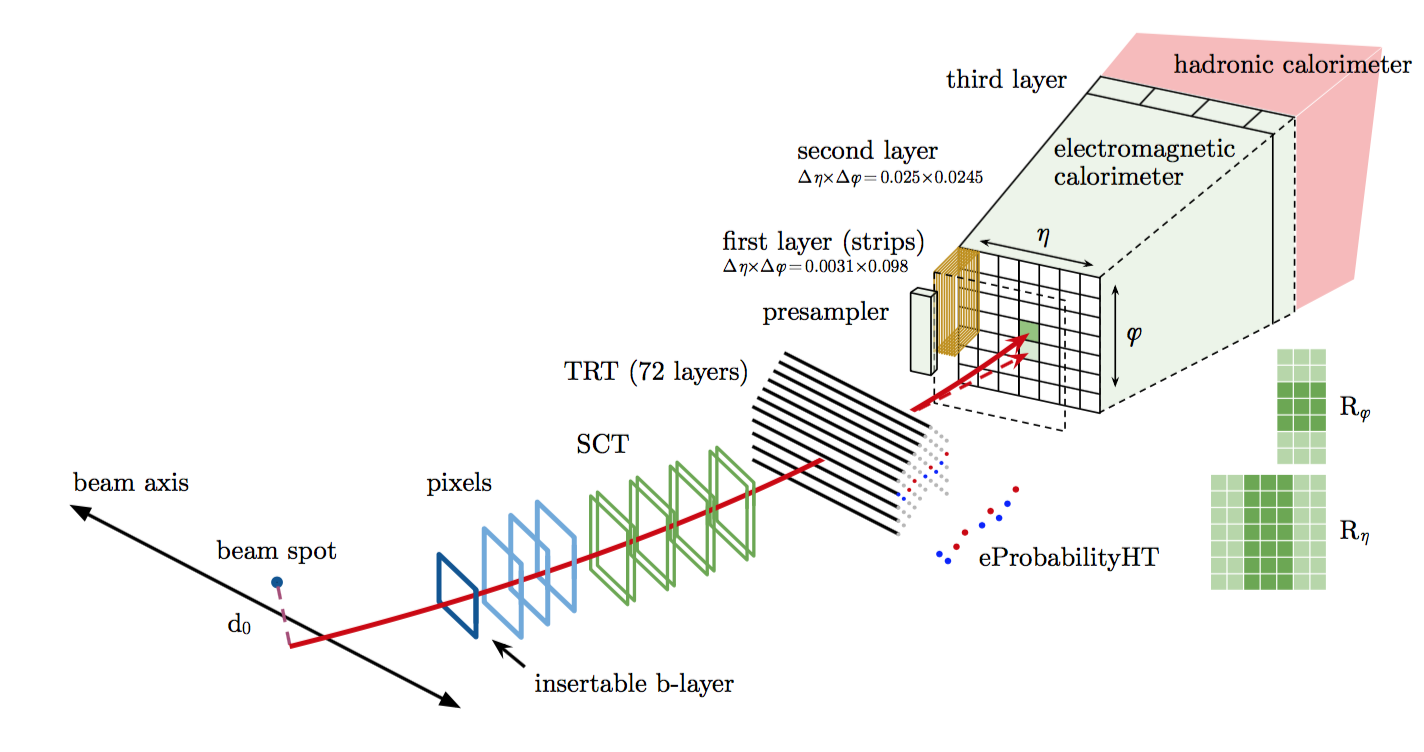
\includegraphics[width=5in]{figures/chapter5/elec_in_detec.png}
    \caption{Schematic depiction of an electron traversing the ATLAS detector.}
    \label{elec_detec}
\end{figure}

%% SUBSECTION: LH
\subsection{The Likelihood Function}
The electron ID algorithm is, at the time of this dissertation, a Likelihood (LH) method; LHs are Multivariate Analysis Techniques used to separate signal from background. This method proceeds in three steps. First, signal and background Probability Density Functions (PDFs) of a set of $n$ variables are constructed from purified samples. The PDFs can be constructed from data or MC simulation depending on the use case; these methods are discussed further in Section \ref{sec:pdfs}. These PDFs can be written as $P_{s,i}(x_i)$ ($P_{b,i}(x_i)$), where s indicates signal and b indicates background. P is the value of the signal (background) PDF of the $i_{th}$ variable evaluated using object $x$. After PDF construction, information from all $n$ variables is combined and all objects are given a discriminant score $d_L$ according to the equation: 
$$d_L=\frac{L_S}{L_S+L_B} \hspace{.5in} L_S(x)=\prod_{i=1}^{n}P_{s,i}(x_i) \hspace{.2in} L_B(x)=\prod_{i=1}^{n}P_{b,i}(x_i).$$
Finally, a cut value on this discriminant is selected and objects which pass this cut are classified as electrons. For the electron LH, the signal and background discriminants peak sharply at 1 and 0 respectively, and so an additional transformation function $d'_L=\tau^{-1}\ln(d_L^{-1}-1)$ is applied to further spread the distributions. The value of $\tau$ is variable and determines the width of the applied spread; $\tau$ is set to 15 for all electron LH calculations. An example of the transformed discriminants can be seen in Figure \ref{fig:trans_disc}.\\

\begin{figure}[hb!]
    \centering
    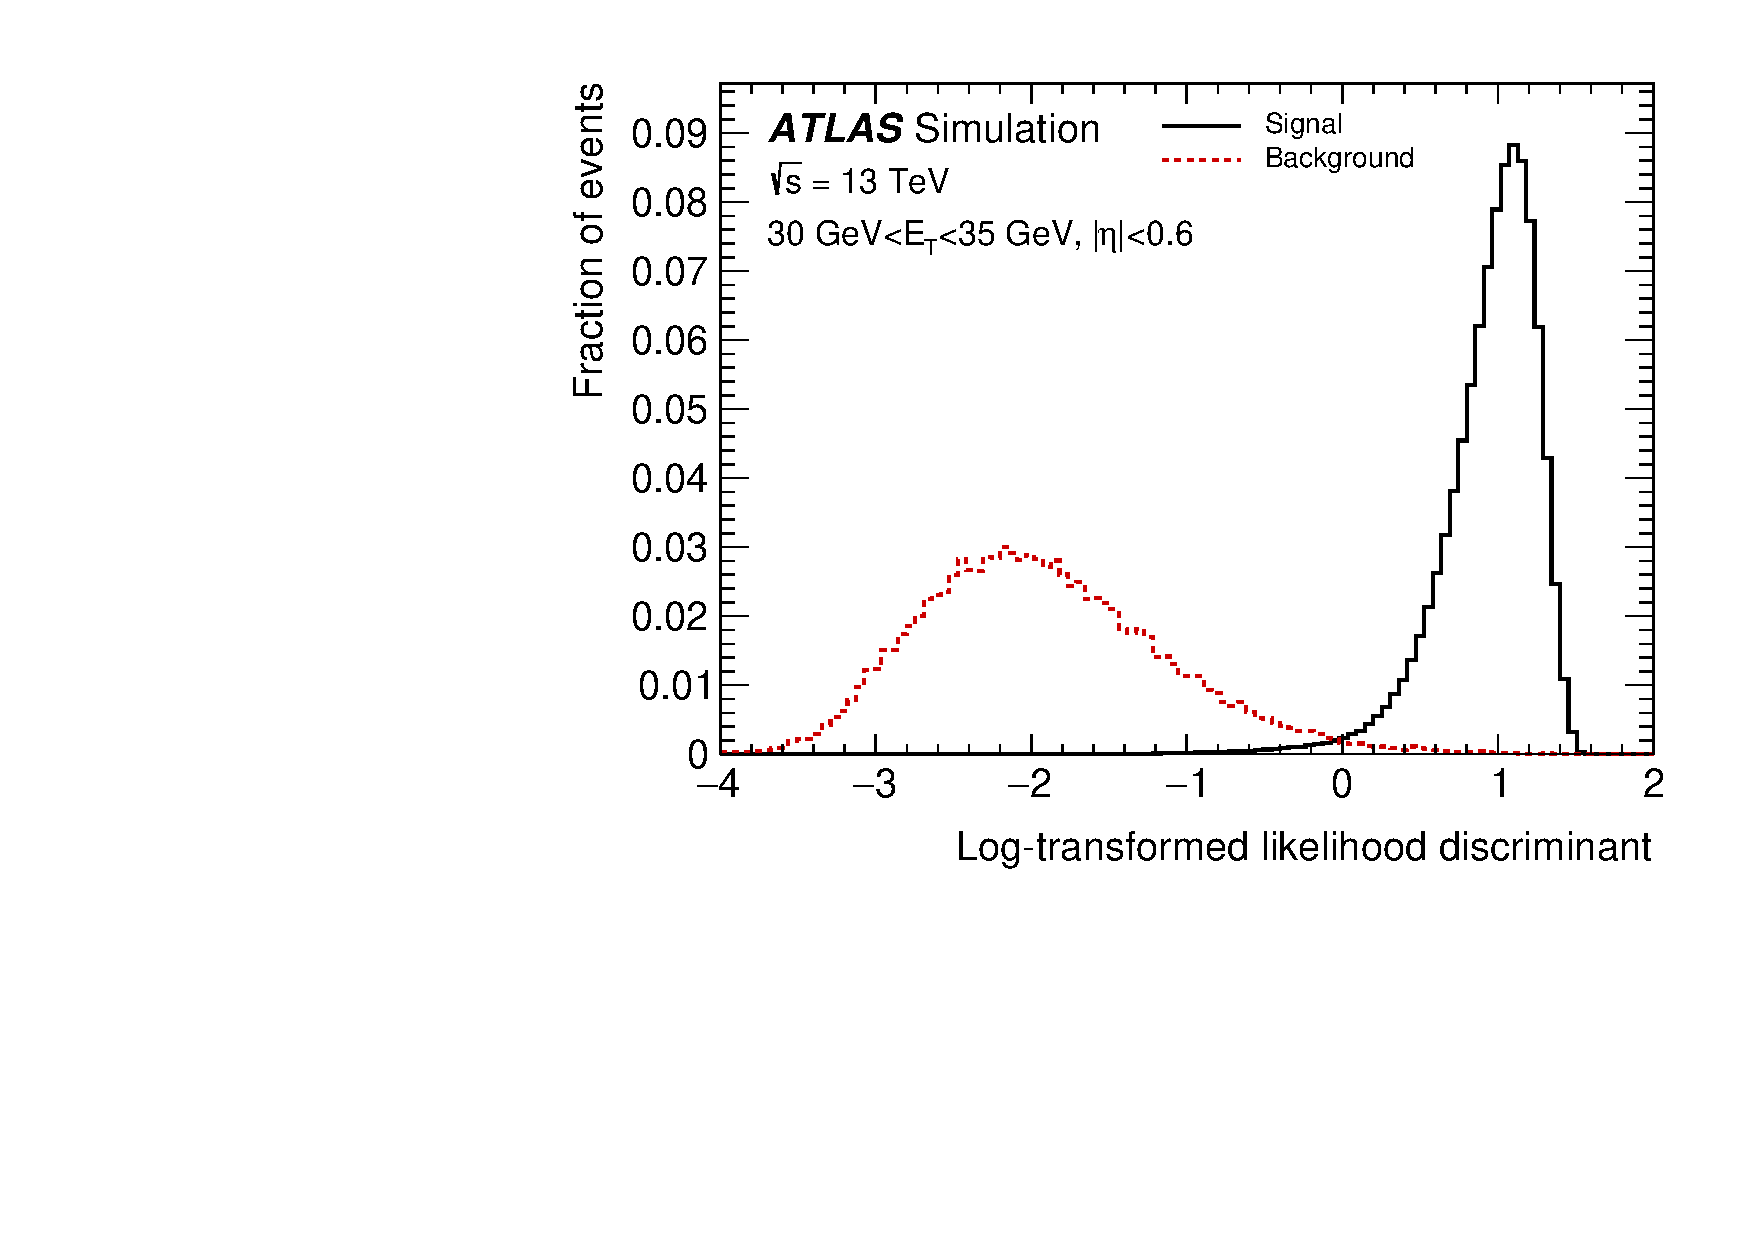
\includegraphics[height=3.5in, angle=270]{figures/chapter5/trans_elec_disc.pdf}
    \caption{The transformed LH-based identification discriminant $d'_L$ for reconstructed electron candidates. The black histogram is for prompt electrons in a $Z\rightarrow ee$ simulation sample, and the red (dashed-line) histogram is for backgrounds in a generic two-to-two process simulation sample (both simulation samples are described in Section \ref{sec:pdfs}). The histograms are normalised to unit area.}
    \label{fig:trans_disc}
\end{figure}

\begin{figure}[hb!]
    \centering
    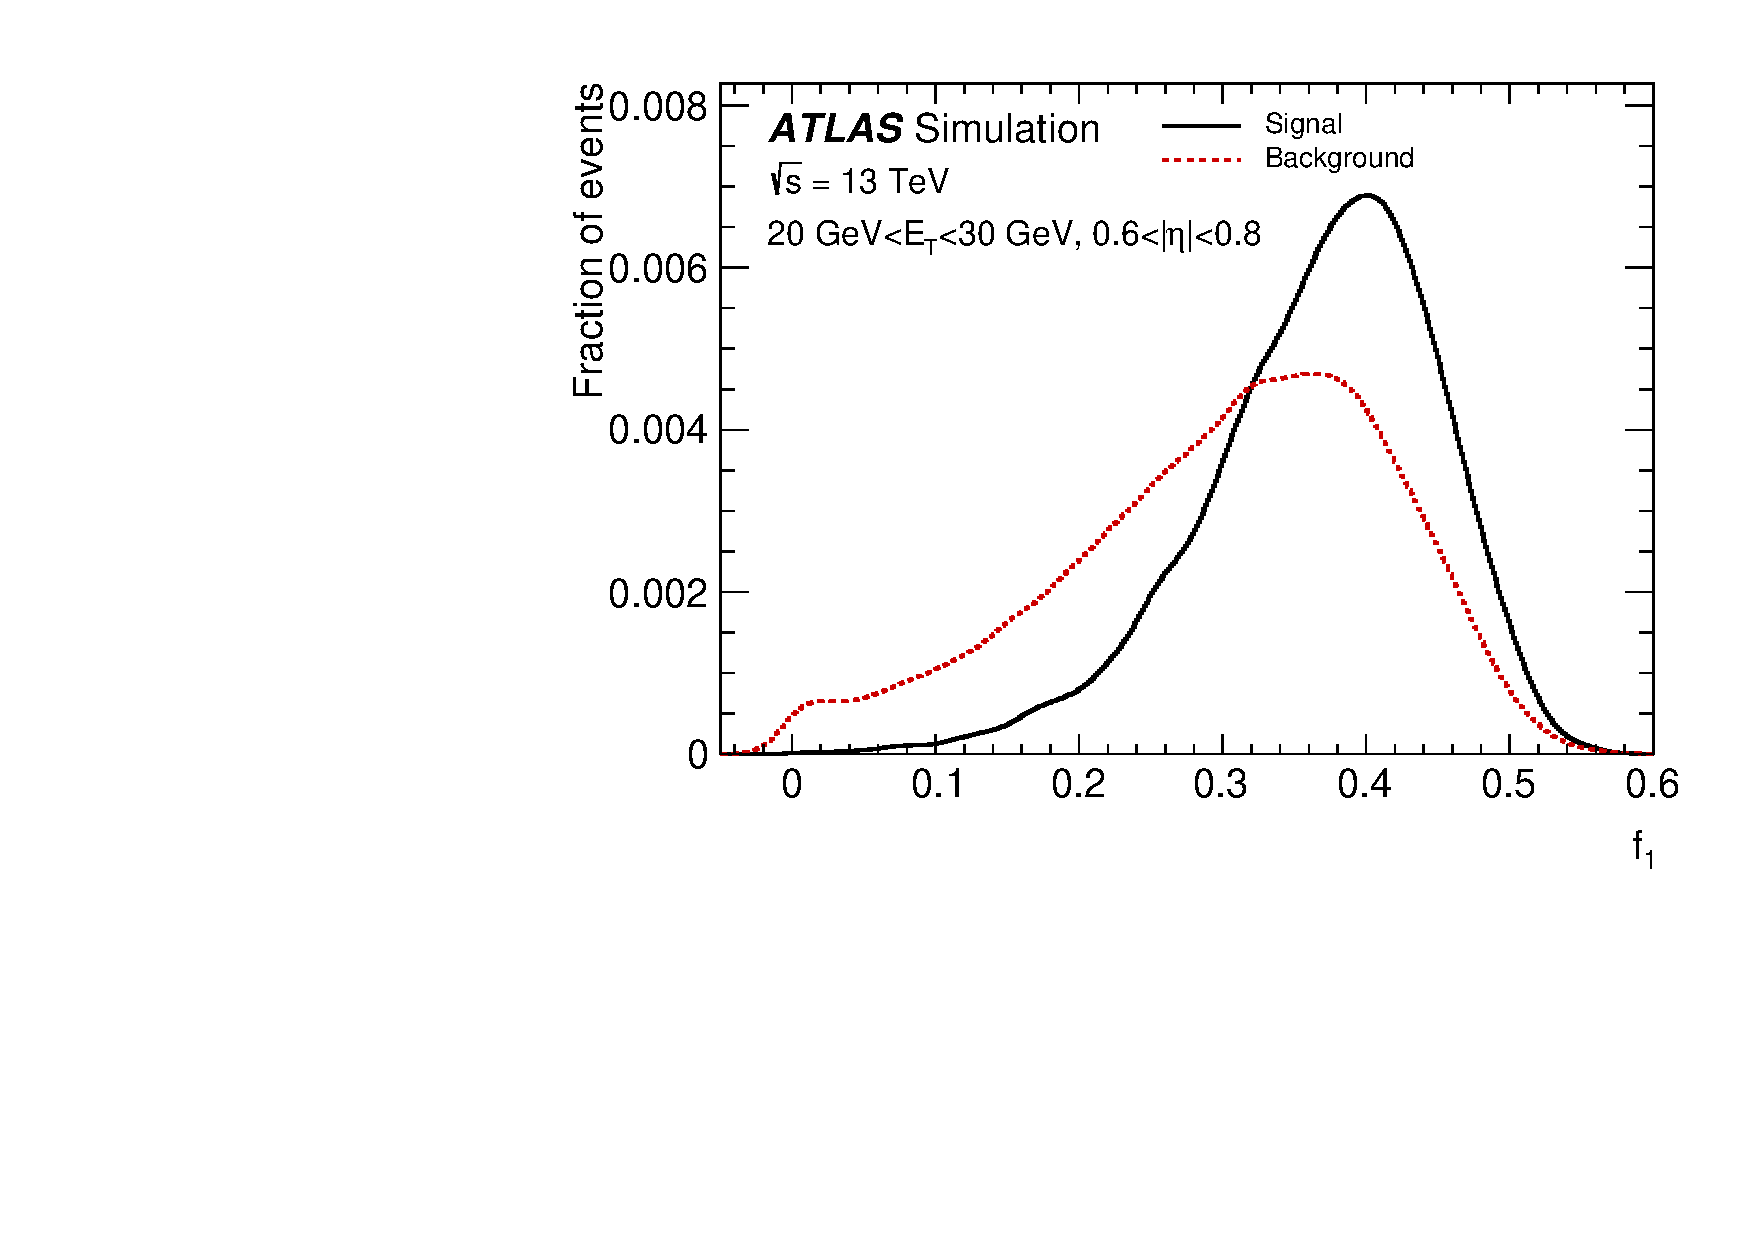
\includegraphics[height=3.5in, angle=270]{figures/chapter5/f1_overlap.pdf}
    \caption{Example of a distribution of an electron variable - $f_1$ described in Table \ref{tab:IDcuts} - that would be inefficient if used in a cut-based ID but improves the LH based ID \cite{run2_elec_paper}.}
    \label{overlap_var}
\end{figure}

A main benefit of the LH method is that it is possible to include variables whose signal and background PDFs overlap in such a way that traditional cut-and-count methods could not be applied, but nonetheless posses discriminating power due to shape or other differences. One such variable, $f_1$, which describes how electrons typically deposit energy in the calorimeter, is shown in Figure \ref{overlap_var}. Additionally, because the LH combines many variables it is able to recover objects from the tails of certain distributions that look reasonable in other PDFs. Together, these effects lead to background rejection up to 2 times more efficient than the Run 1 cut-based algorithm (see Figure \ref{cut_to_lh}).\\ 


\begin{figure}[h!]
    \begin{subfigure}
        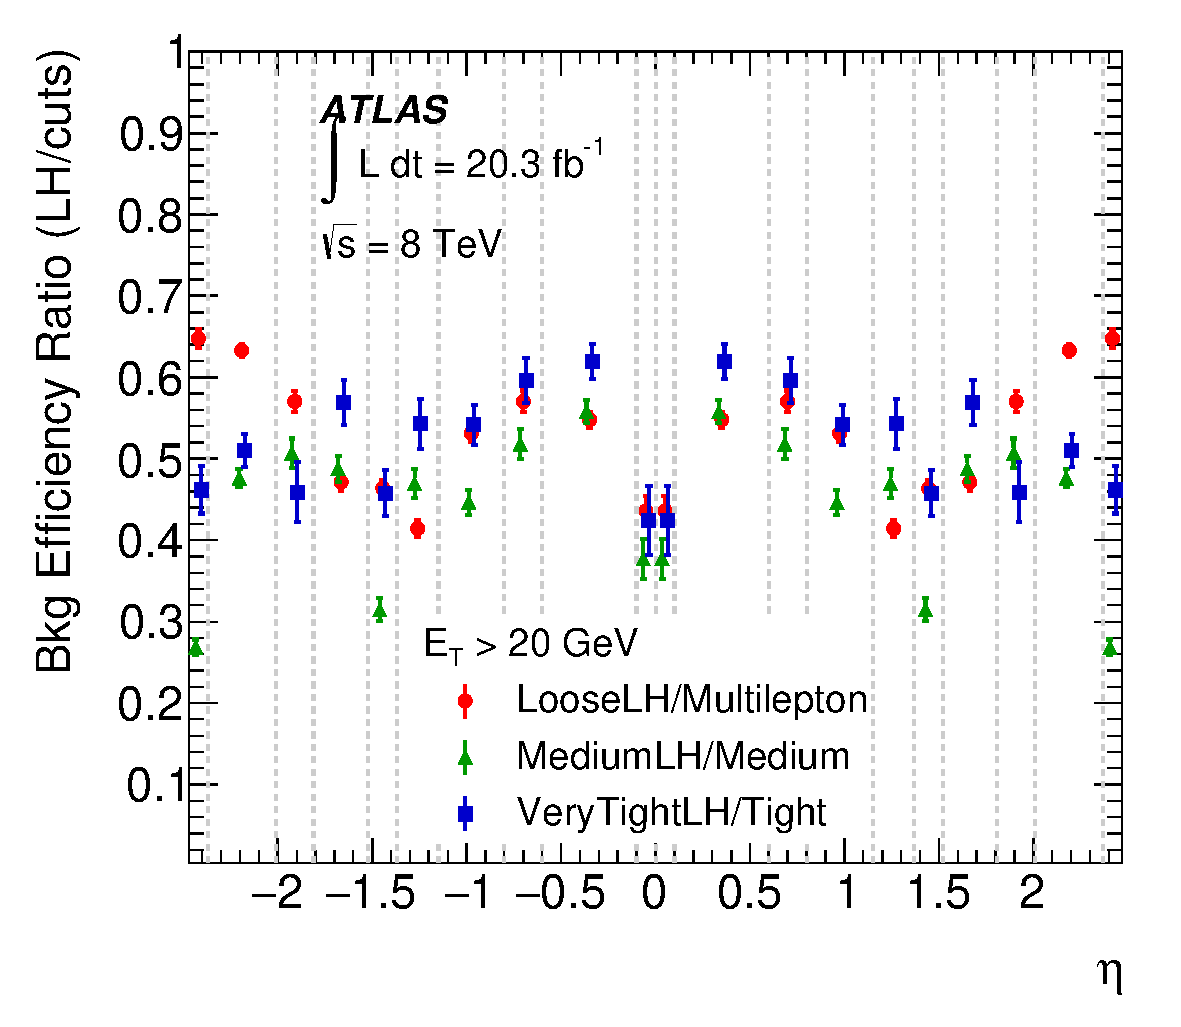
\includegraphics[width=3in]{figures/chapter5/lh_to_cut_eta.pdf}
    \end{subfigure}
    \begin{subfigure}{
        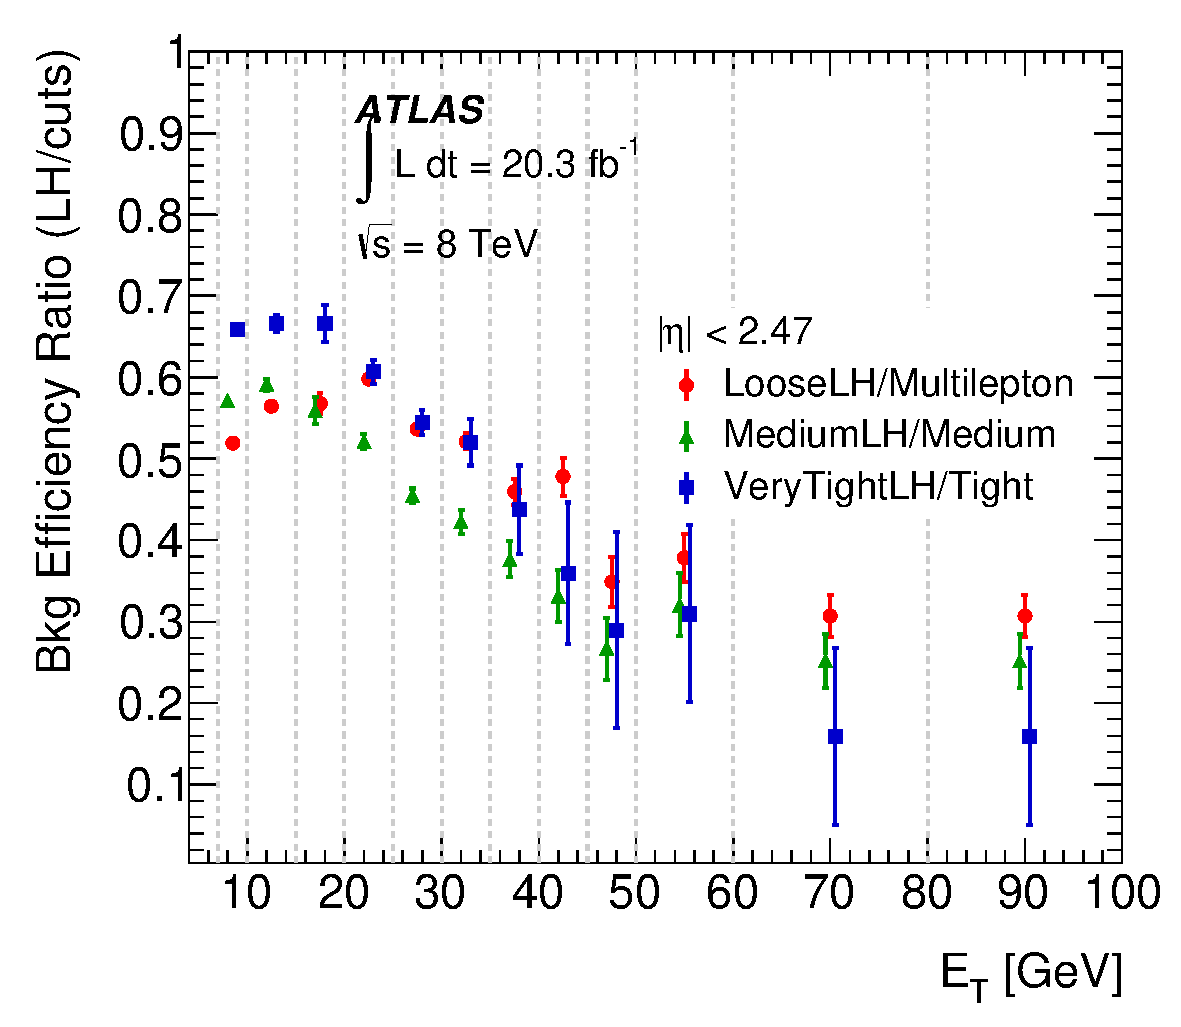
\includegraphics[width=3in]{figures/chapter5/lh_to_cut_pt.pdf}
    \end{subfigure}
    \caption{Ratio of background efficiencies for a LH based algorithm to that of the closest-efficiency cut-based selections as a function of $\eta$ (left) and $E_T$ (right) \cite{run1_elec_paper}.}
    \label{cut_to_lh}
\end{figure}

\pagebreak

During the original Run 1 development of the LH-based ID, other ML algorithms including BDTs and NNs were considered. Ultimately, the LH technique was selected due to its simplicity, interpretability, and processing speed \cite{lh_paper}. In order to improve the electron ID efficiency for full Run 2 analyses and future Run 3 and HL-LHC analyses, more complex ML techniques are being studied. This is described further in Section \ref{ml_id}.

%% SUBSECTION: Electron LH
\subsubsection{Electron Likelihood}\label{elec_lh}
The electron LH ID uses a combination of up to 19 detector related variables. The motivation for these variables is described below, and a summary can be found in Table \ref{tab:IDcuts}. \\

\begin{table*}
\begin{adjustwidth}{-1in}{-1in}
\caption{Definitions of electron discriminating variables, the types of backgrounds the variables help to discriminate against (light-flavor (LF), converted photons ($\gamma$), or heavy-flavor (HF)), and if a variable is used as a likelihood PDF ($\mathcal{L}$) or used as a rectangular cut (C). The $^{*}$ refers to the fact that the $E/p$ and $w_{stot}$ variables are
only used for electrons with $p_T > 150$ GeV for the Tight identification operating point, and are not used for the looser operating points.}
\label{tab:IDcuts}
\footnotesize
\begin{center}
\begin{tabular}{|l|l|l|c|c|c|l|}
\hline
Type & Description & Name &  \multicolumn{3}{c|}{Rejects} & Usage  \\
& & & LF & $\gamma$ & HF &\\
\hline
Hadronic & Ratio of $E_T$ in the first layer of the hadronic calorimeter  & $R_{had1}$ & x & & x & $\mathcal{L}$ \\ 
leakage & to $E_T$ of the EM cluster. & & & & & \\
& (used over the range $|\eta| < 0.8$ or $|\eta| > 1.37$)  & & & & & \\
\cline{2-7}
& Ratio of $E_T$ in the hadronic calorimeter &  & & & & \\
&  to $E_T$ of the EM cluster. & $R_{had}$ & x & & x & $\mathcal{L}$  \\
& (used over the range $0.8 <|\eta| < 1.37$) & & & & & \\
\hline
Back layer of  & Ratio of the energy in the back layer to the total energy in the & & & & &\\
EM calorimeter & EM accordion calorimeter. This variable is only used for & & & & & \\
               & $p_T < 80$ GeV due to known inefficiencies at high $p_T$, and is& $f_3$ & x & & & $\mathcal{L}$ \\
             & also removed from the LH for $|\eta| > 2.37$, where it is& & & & & \\
              & poorly modeled by the MC. & & & & & \\
\hline
Middle layer of  & Lateral shower width, $\sqrt{(\Sigma E_i \eta_i^2)/(\Sigma E_i) -((\Sigma E_i\eta_i)/(\Sigma E_i))^2}$, & & & & & \\
EM calorimeter  & where $E_i$ is the energy and $\eta_i$ is the pseudorapidity  & $w_{\eta 2}$ & x & x & & $\mathcal{L}$ \\
& of cell $i$ and the sum is calculated within a window of $3\times5$ cells & & & & & \\
\cline{2-7}
& Ratio of the energy in 3$\times$3 cells over the energy in 3$\times$7 cells & $R_{\phi}$ & x & x & x & $\mathcal{L}$  \\
& centered at the electron cluster position & & & & & \\
\cline{2-7}
& Ratio of the energy in 3$\times$7 cells over the energy in 7$\times$7 cells  & $R_{\eta}$ & x & x & x & $\mathcal{L}$  \\
& centered at the electron cluster position & & & & & \\
\hline
Strip layer of       & Shower width, $\sqrt{(\Sigma E_i (i-i_\mathrm{max})^2)/(\Sigma E_i)}$, where $i$ runs over  &   & & & & \\ 
EM calorimeter       & all strips in a window of $\Delta\eta \times \Delta\phi \approx 0.0625 \times 0.2$,  & $w_{stot}$ & x & x & x & C$^{*}$ \\
                     & corresponding typically to 20 strips in $\eta$, & & & & &                  \\
                     & and $i_\mathrm{max}$ is the index of the highest-energy strip        &  & & & &   \\
\cline{2-7}
                     & Ratio of the energy difference between the maximum &    & & & &  \\
                     & energy deposit and the energy deposit in a secondary & $E_{ratio}$ & x & x & & $\mathcal{L}$  \\
                   & maximum in the cluster to the sum of these energies & & & & &   \\
\cline{2-7}     
& Ratio of the energy in the strip layer to the total energy  & $f_1$ & x & & & $\mathcal{L}$  \\
	& in the EM accordian calorimeter &  & & & & \\
\hline
Track  & Number of hits in the innermost pixel layer;&   $n_\mathrm{Blayer}$ & & x & & C \\
conditions & discriminates against photon conversions &   $ $  & & & & \\
	\cline{2-7}
	                     & Number of hits in the pixel detector        &    $n_\mathrm{Pixel}$ & & x & & C \\
	\cline{2-7}
                     & Number of total hits in the pixel and SCT   detectors  &   $n_{\mathrm{Si}}$  & & x & & C \\
	\cline{2-7}
                     & Transverse impact parameter with respect to the beam-line
                     &       $d_0$  & & x & x & $\mathcal{L}$ \\
\cline{2-7}
                     & Significance of transverse impact parameter & $|{d_0/\sigma_{d_0}}|$  & & x & x & $\mathcal{L}$  \\
                   & defined as the ratio of $d_0$ and its uncertainty                     &  & & & &              \\
\cline{2-7}
                     &  Momentum lost by the track between the perigee and the last &  $\delta p/p$ & x & & & $\mathcal{L}$ \\
                   & measurement point divided by the original momentum & & & & & \\
\hline
TRT                       & Likelihood probability based on transition radiation in the TRT &   $eProbabilityHT$ & x & & & $\mathcal{L}$  \\
	\hline
Track-cluster     & $\Delta\eta$ between the cluster position in the strip layer &   $\Delta \eta_1$ & x & x & & $\mathcal{L}$  \\
matching          &  and the extrapolated track & & & & &   \\
\cline{2-7}
&   $\Delta\phi$ between the cluster position in the middle layer &   & & & &  \\
&   of the calorimeter and the track extrapolated from the middle & & & & & \\
& layer to the perigee, where the track momentum is rescaled  to & $\Delta \phi_{res}$ & x & x & & $\mathcal{L}$  \\
&   the cluster energy before extrapolating  & & & & &  \\
\cline{2-7}
                    & Ratio of the cluster energy to the track momentum            &       $E/p$   & x & x & & C$^{*}$\\ 
\hline
\end{tabular}
\end{center}
\end{adjustwidth}
\end{table*}

$R_{had}$, the ratio of energy deposited in the handronic calorimeter to energy in the electromagnetic calorimeter distinguish electrons from hadrons based on how far they traverse through the detector. Calorimeter shower width variables $w_{stot}$, $w_{\eta}_2$, $R_{\eta}$, and $R_{\phi}$ further separate electrons and hadrons as hadrons typically have much wider showers than electrons. Additionally, the other calorimeter depth variables $f_1$ and $f_3$ describe shower shapes as the object proceeds through the electromagnetic calorimeter.  $E_{ratio}$ checks for multiple incident particles by comparing the difference in the two largest energy clusters in the silicon strip layer of the electromagnetic calorimeter to their sum. \\

Variables $d_0$ and $|d_0/\sigma d_0|$ describe the object's transverse and longitudinal impact parameters which helps distinguish possible electrons from b- and c-jets. $\Delta p /p$ characterizes an object's bremsstrahlung radiation loss and separates electrons from charged hadrons which lose much less energy in the Inner Detector. \\

Finally, the variable $eProbabilityHT$ exploits transition radiation information from the TRT. Light objects like electrons radiate more photons in the TRT than heavier objects like pions and muons, and the radiated photons produce additional high-threshold (HT) hits in the TRT. In Run 1, the variable $F_{HT}$, or the ratio of HT hits to total TRT hits was used in the electron LH. Leaks in the TRT gas system necessitated replacement of several xenon modules with argon modules and resulted in a decreased probability of HT hits in the TRT. Consequently, a tool was developed to regain the information from the original $F_{HT}$ variable. The HT probability of each TRT hit is calculated using the electron hypothesis and pion hypothesis separately. $eProbabilityHT$ describes the ratio of these two probabilities. The development and implementation of this tool is described in further detail in \cite{2015_eff_paper}. \\


The distributions of the variables described above vary with both particle $E_T$ and $\eta$. Consequently, PDFs and LHs are constructed separately for a 10x9 set of $p_T$ and $\eta$ bins. The $\eta$ bin limits are taken from the detector geometry and the $p_T$ bin limits were set after a study of the rate of shower-shape change. The bin definitions are shown in Tables \ref{tab:etbins} and \ref{tab:etabins}.\\

\begin{table*}[!htbp]
	\begin{center}
	\begin{tabular}{l|ccccccccccc}
	\hline
	\multicolumn{12}{c}{Bin boundaries in $p_T$ [GeV]}\\
	\hline
	PDFs                    & 4.5& 7& 10& 15& 20& 30& 40& $\infty$&  &   & \\
	\hline
	\end{tabular}
	\end{center}
	  \caption{Electron transverse energy binning used for the electron likelihood PDFs and discriminant cut values.}
	\label{tab:etbins}	
\end{table*}

\begin{table*}[!htbp]
\begin{center}
\begin{tabular}{cccccccccc}
\hline
\multicolumn{10}{c}{Bin boundaries in $|\eta|$}\\
\hline
0.0& 0.6& 0.8& 1.15& 1.37& 1.52& 1.81& 2.01& 2.37& 2.47 \\
\hline
\end{tabular}
\end{center}
\caption{Electron pseudorapidity binning used for the electron likelihood PDFs and discriminant cut values.}
\label{tab:etabins}
\end{table*}

The LH ID is used both in offline data processing and online for HLT electron triggers. The trigger LH differs from the offline algorithm described above in a few small ways. First, the $\Delta p/p$ variable is not used in the HLT because the track-fitting algorithm is too computationally intensive. Furthermore, impact parameter variables $d_0$ and $|d_0/\sigma d_0|$ are not used to allow analyses which rely on leptonically decaying $\tau$ leptons or other exotic particles (such as the VH,H$\rightarrow\tau\tau$ described in Chapters 6 and 7) to also utilize the HLT electron triggers. Finally, PDFs for the HLT LH are constructed separately due to different variable resolutions compared to the offline ID. An additional HLT LH ID exists which uses only calorimeter variable information. This ID is used as a highly efficient preselection before track reconstruction algorithms are run; events which fail this preselection do not undergo track finding, reducing the amount of computational resources needed. 

%% SUBSECTION:  OPs
\subsubsection{Operating Points}
The electron ID LH is used to support five operating points which provide ATLAS analyses flexibility to balance signal selection efficiency and background rejection. These operating points are referred to as Very Loose, Loose, LooseAndBLayer, Medium, and Tight. Background rejection efficiency increases from the VeryLoose to Tight operating points and each operating point is a subset of all looser operating points.\\

The LH discriminant cut defining each operating point was initially selected in Run 1 to reproduce the efficiency of the original cut-based electron ID. Subsequent retunings and developments of the LH algorithm have sought to maintain roughly these same efficiencies while further improving background rejection. The VeryLoose operating point was added in Run 2 primarily for use in background estimation techniques that benefit from a reduced electron ID (such as the Fake Factor Method described in Chapter 7).\\

In addition to passing the LH discriminant cut for each operating point, electron candidates are also required to pass good track-quality requirements of at least one pixel hit and at least seven silicon hits to be classified as an electron. The Loose, Medium, and Tight operating points require an additional pixel hit to reduce the contribution of converted photons. To further remove conversions, the Medium and Tight operating points require a hit in the inner-most pixel layer, the IBL. The LooseAndBLayer operating point was designed to include this additional requirement while maintaining the Loose operating point efficiency. The efficiency of the Loose, Medium, and Tight operating points for 2017 data and MC can be seen in Figure \ref{fig:2017_eff}. The efficiency is slightly higher for MC due to the tuning procedure which incorporates pile-up profiles derived from MC as described in \cite{id_note}. This discrepancy is accounted for the the data to MC correction scale factors.\\

\begin{figure}[h]
    \begin{subfigure}
        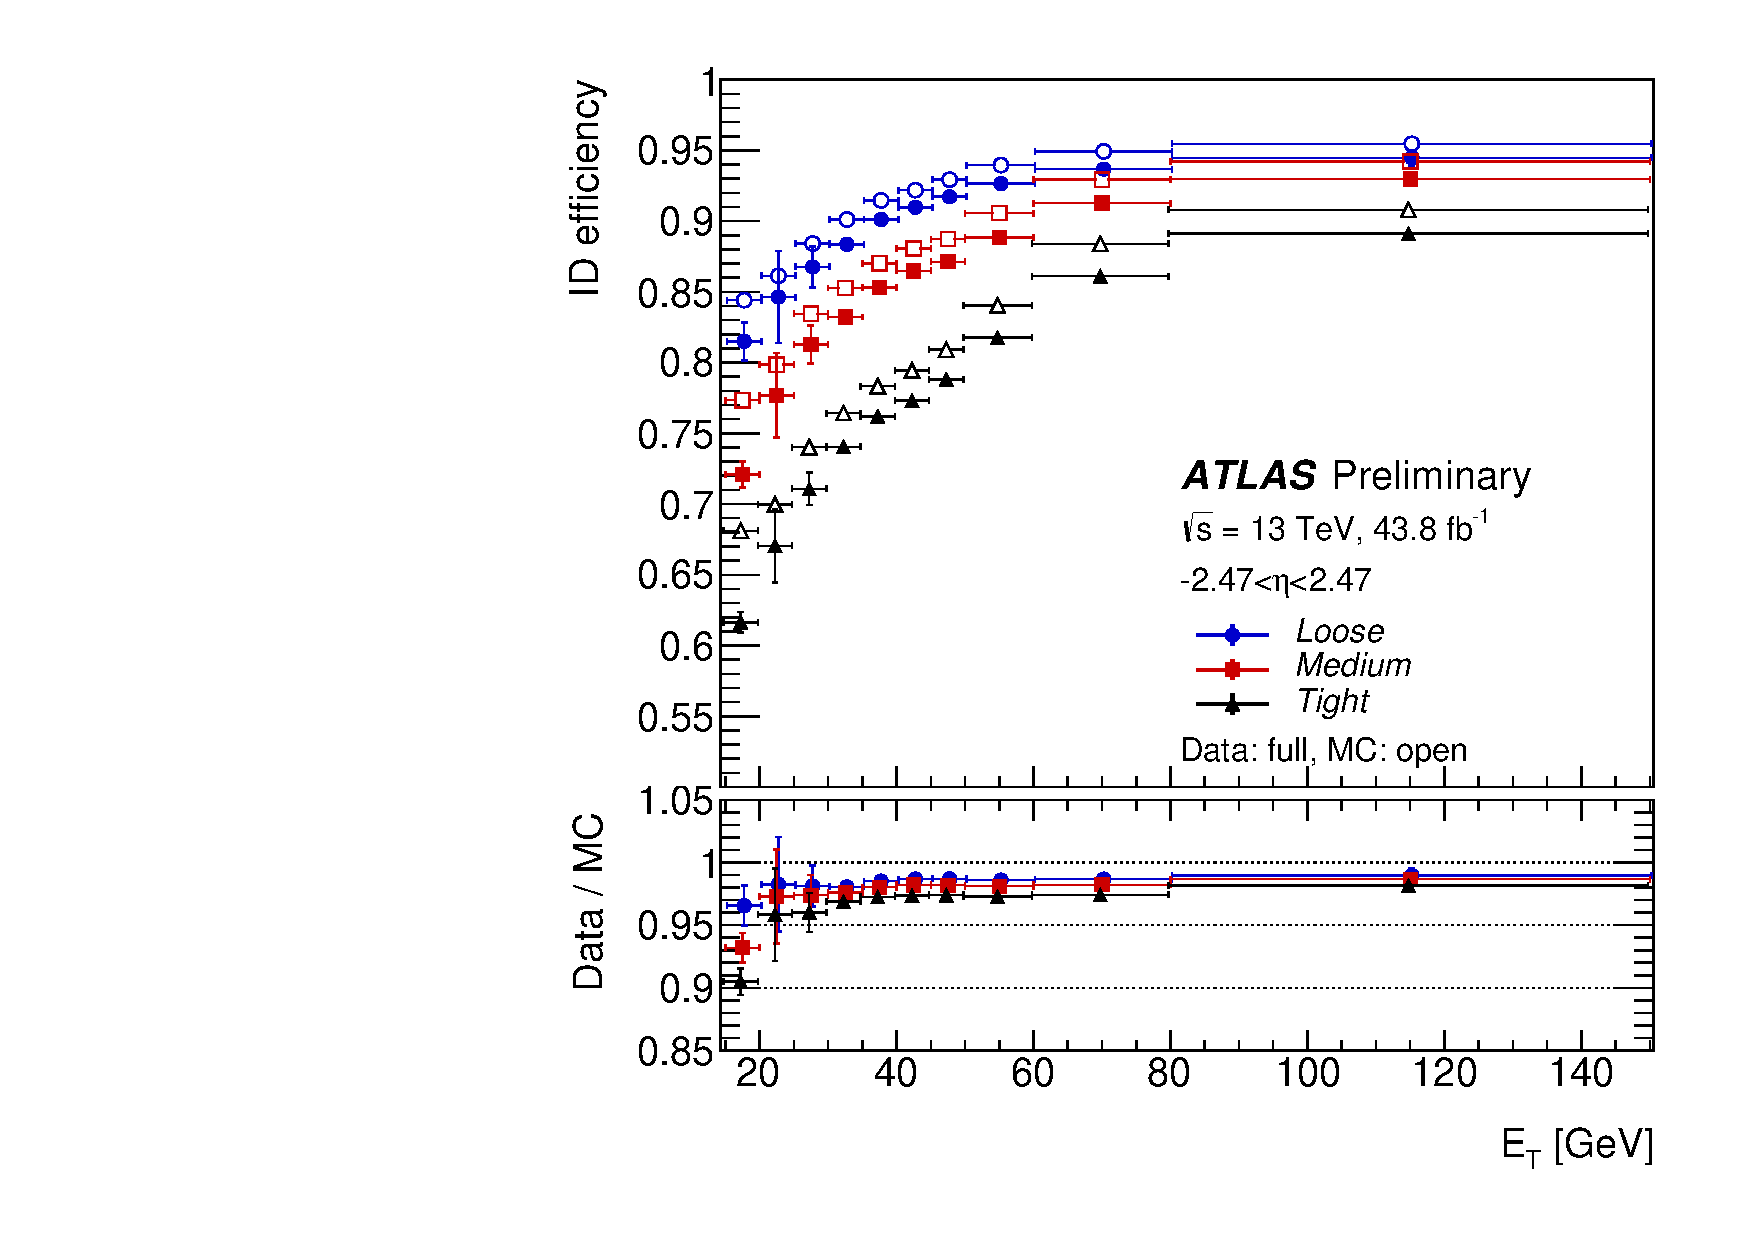
\includegraphics[width=2.5in, angle=270]{figures/chapter5/elec_op_eff_pt.pdf}
    \end{subfigure}
    \begin{subfigure}
        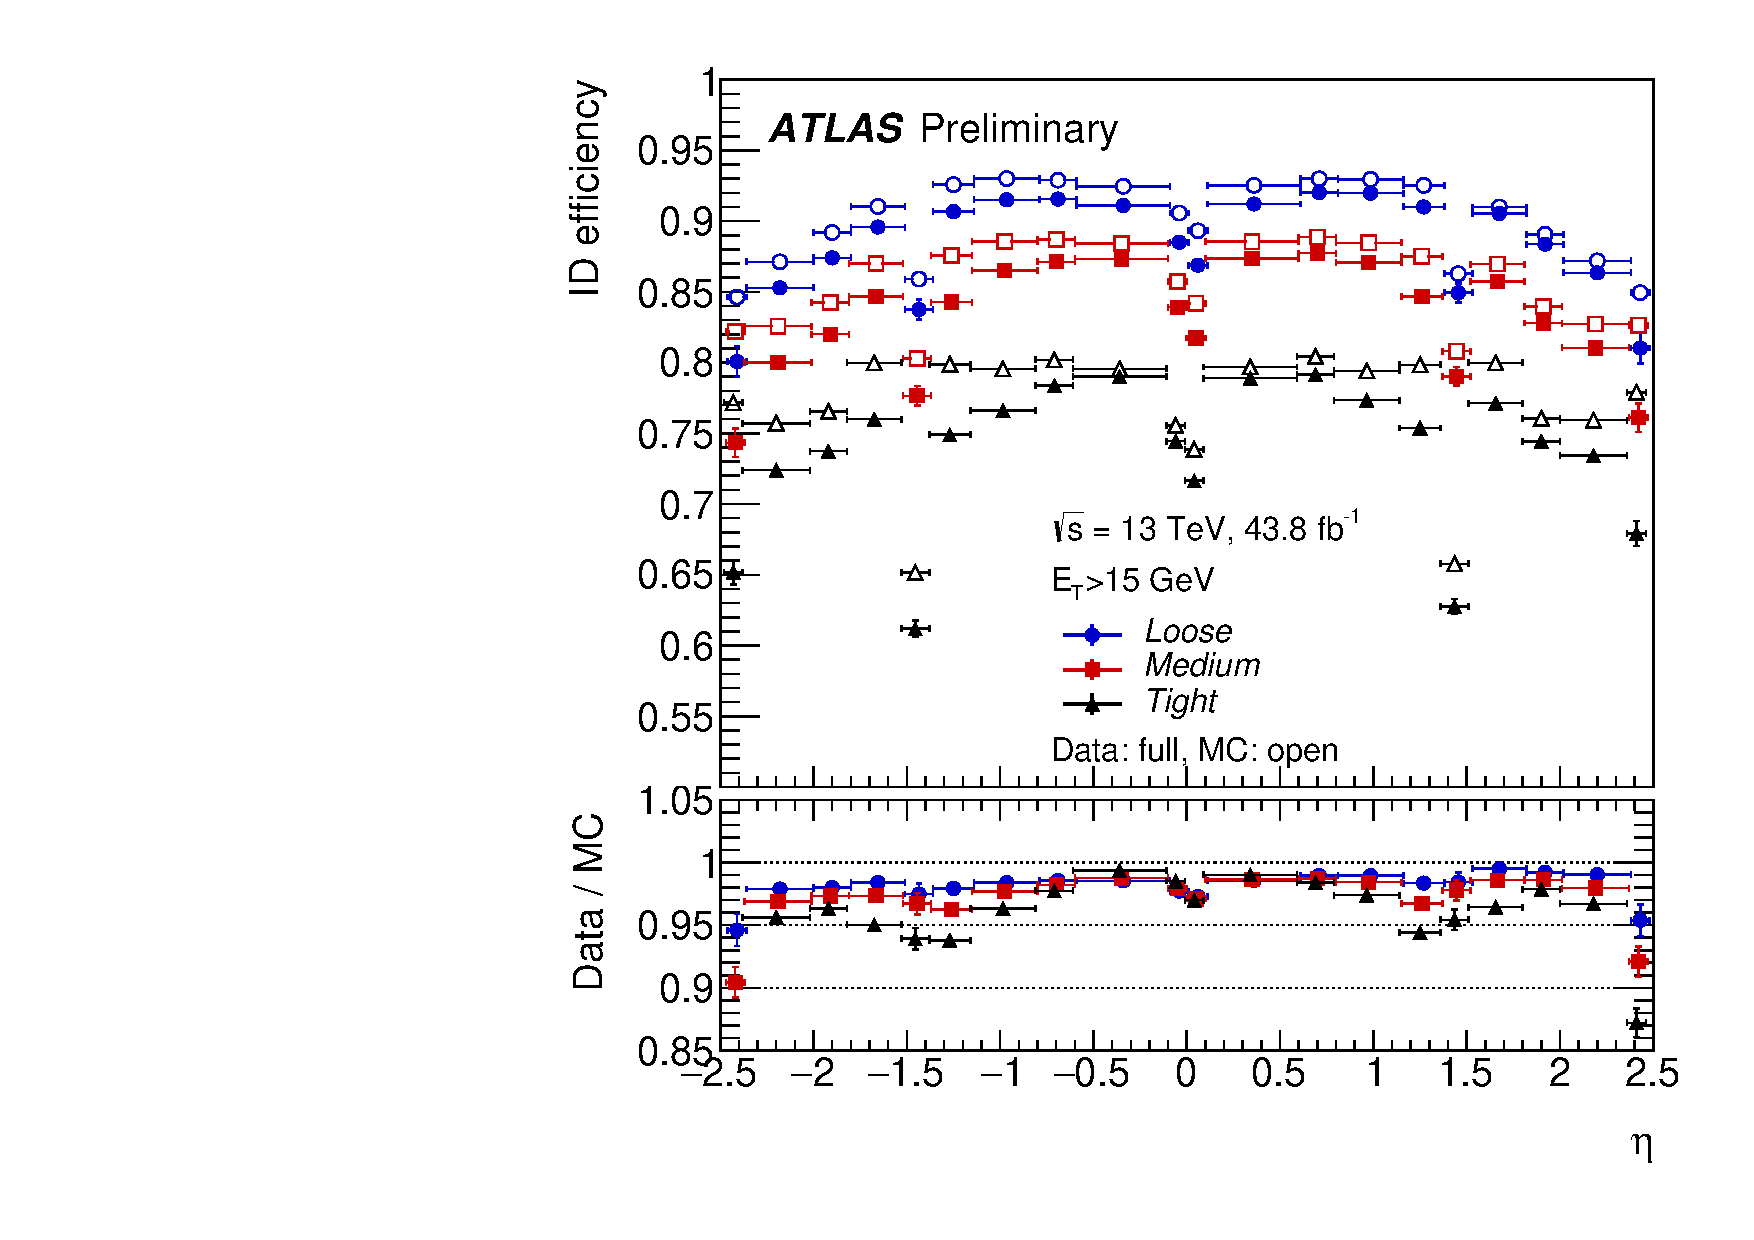
\includegraphics[width=2.5in, angle=270]{figures/chapter5/elec_op_eff_eta.pdf}
    \end{subfigure}
    \caption{Electron identification efficiencies for $Z\rightarrow ee$ events as a function of $E_T$ (left) and pseudo-rapidity (right). The efficiencies are shown for data (full) and MC (open) for three LH based operating points \cite{eff_plots}.}
    \label{fig:2017_eff}
\end{figure}

%% SUBSECTION: PDFs
\subsection{Probability Density Functions (PDFs)}\label{sec:pdfs}
The PDFs used to build the LH ID are constructed from either MC of relevant processes or purified data samples. An individual PDF is created by building a histogram of a single variable for the entire MC or data sample; all variables used are described in Section \ref{elec_lh}. Signal PDFs are constructed using the Tag-and-Probe method described below, while background PDFs are constructed from objects which pass one of the electron/photon supporting triggers. Additional cuts ($M_T<40$ GeV, $MET<25$ GeV) are included to remove any objects resulting from W decays, and an invariant-mass $<40$ GeV or $>140$ GeV) cut is included to remove contributions from Z decays.\\

\subsubsection{Tag \& Probe Method}
In order to increase purity in the signal electron ID PDFs while maintaining unbiased electron candidates, a Tag \& Probe method is used to construct the final PDFs from the original sample. With this method, developing a new set of ID operating points relies on the previous iteration. \\

All ID PDFs are constructed using electrons from processes where an object (a Z boson or a $J/\psi$ meson) decays into two electrons. After event level selections for the relevant process are applied, one of the electrons (the ``tag") is required to pass the Tight operating point. A second electron in the event which, when combined with the tag electron, forms an invariant mass within 10 GeV (.3 GeV) of the Z mass ($J/\psi$ mass) is then labeled the ``probe" electron. The probes are thus unbiased and used to build the LH PDFs. A full list of event selection and Tag \& Probe level cuts can be found in Table \ref{tab:tp_Z} for $Z\rightarrow ee$ and Table \ref{tab:tp_J} for $J/\psi \rightarrow ee$. Additional details regarding the Tag \& Probe method for $J/\psi\rightarrow ee$ events can be found in Section \ref{low_pt_sec} and the overall method is further described in \cite{run1_elec_paper} and \cite{id_note}.

\begin{table}[h]
\footnotesize
\renewcommand{\arraystretch}{1.3}
\begin{center}
\begin{tabular}{l}
\textbf{Tag \& Probe Selection for $Z\rightarrow ee$ events} \\
\hline
Single electron trigger fired \\
\midrule
 Tag electron with $p_T > 25~GeV$ \\
	    Tag electron $|\eta| < 1.37$ OR $(|\eta| > 1.52$ AND $|\eta| < 2.47)$ \\
	    Tag electron passes Tight identification \\
	    $\Delta$R(tag electron, trigger electron) $<$ 0.10 \\
	    Tag electron passes LAr object quality requirement \\
	\midrule
	    Probe electron with $p_T > 15~GeV$ \\
	    Probe electron $|\eta| < 2.47$ \\
	    Probe electron passes VeryLoose identification \\
	    Probe electron passes LAr object quality requirement \\
	\midrule
	    $80~GeV < m_{ee} < 100~ GeV$ \\
	    Tag electron and probe electron have opposite electric charge \\
	\hline
	\end{tabular}
	\end{center}
	  \caption{Summary of Tag \& Probe selection for $Z\rightarrow ee$ events}
	\label{tab:tp_Z}
	\end{table}

\begin{table}[h]
\footnotesize
\renewcommand{\arraystretch}{1.3}
\begin{center}
\begin{tabular}{l}
\textbf{Tag \& Probe Selection for $J/\psi\rightarrow ee$ events.} \\
\hline
Di-electron trigger fired\\
\midrule
Tag electron with $p_T > 4.5~GeV$ \\
    Tag electron $|\eta| < 1.37$ OR $(|\eta| > 1.52$ AND $|\eta| < 2.47)$ \\
	    Tag electron passes Tight identification \\
	    $\Delta$R(tag electron, trigger electron) $<$ 0.10 \\
	    Tag electron passes LAr object quality requirement \\
	\midrule
    Probe electron with $p_T > 4.5~GeV$ \\
	    Probe electron $|\eta| < 2.47$ \\
	    Probe electron passes VeryLoose identification \\
	    Probe electron passes LAr object quality requirement \\
	\midrule
	    $2.8~GeV < m_{ee} < 3.3~GeV$ \\
	    Tag electron and probe electron have opposite electric charge \\
	    $\Delta$R(tag electron, probe electron) $>$ 0.10 \\
	    $-1 < \tau < 0.2$\\
	\hline
\end{tabular}
\end{center}
\caption{Summary of Tag \& Probe selection for $J/\psi\rightarrow ee$ events.}
\label{tab:tp_J}
\end{table}

%% subsec: smoothing
\subsubsection{Smoothing PDFs}
The PDFs used to construct the LH should contain only physically meaningful features and be free of fluctuations due to binning and statistics. Low statistics in a particular PDF could cause similar electron candidates to be assigned vastly different final discriminant values, and in particular a bin with 0 value would lead to undefined discriminates for some electron candidates. To mitigate these issues, Adaptive Kernel Density Estimation (KDE) is applied to all signal and background PDFs before the final LH discriminant is calculated. \\

KDE serves to smooth a variable distribution by treating each bin in the PDF as a $\delta$-function, replacing each $\delta$-function with a ``kernel" function, then summing all the kernel functions to form the final PDF. For the purposes of the LH ID, the kernel function is a Gaussian with a tunable width parameter. In the adaptive KDE method, the Gaussian width parameter is increased in bins with low statistics. A visualization of both methods is presented in Figure \ref{fig:kde}, along with an example of a smoothed and unsmoothed PDF. The electron LH PDFs are smoothed using the TMVA adaptive KDE tool \cite{tmva}.

\begin{figure}[hb!]
\begin{subfigure}
    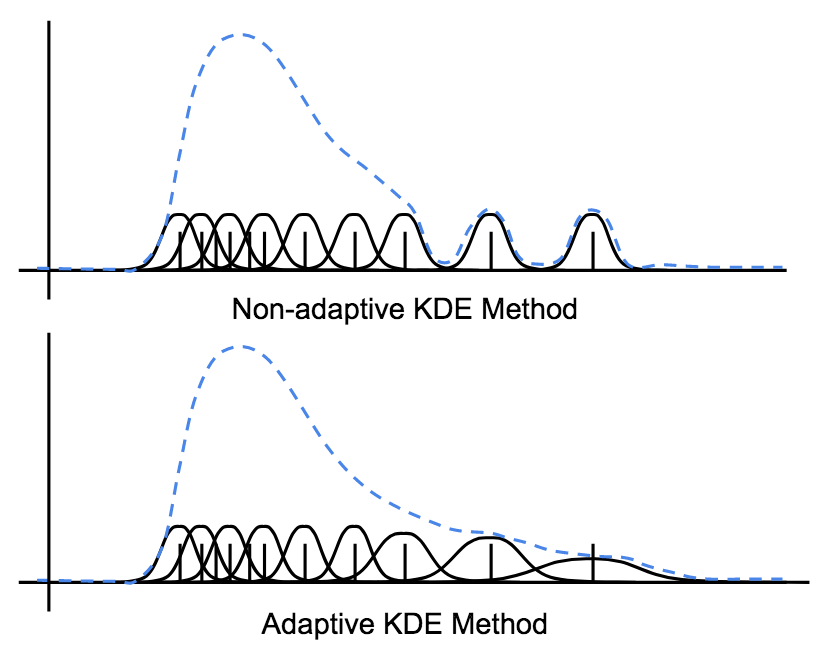
\includegraphics[width=2.5in, height=2.5in]{figures/chapter5/kde_method.pdf}
    \centering
\end{subfigure}
\begin{subfigure}
    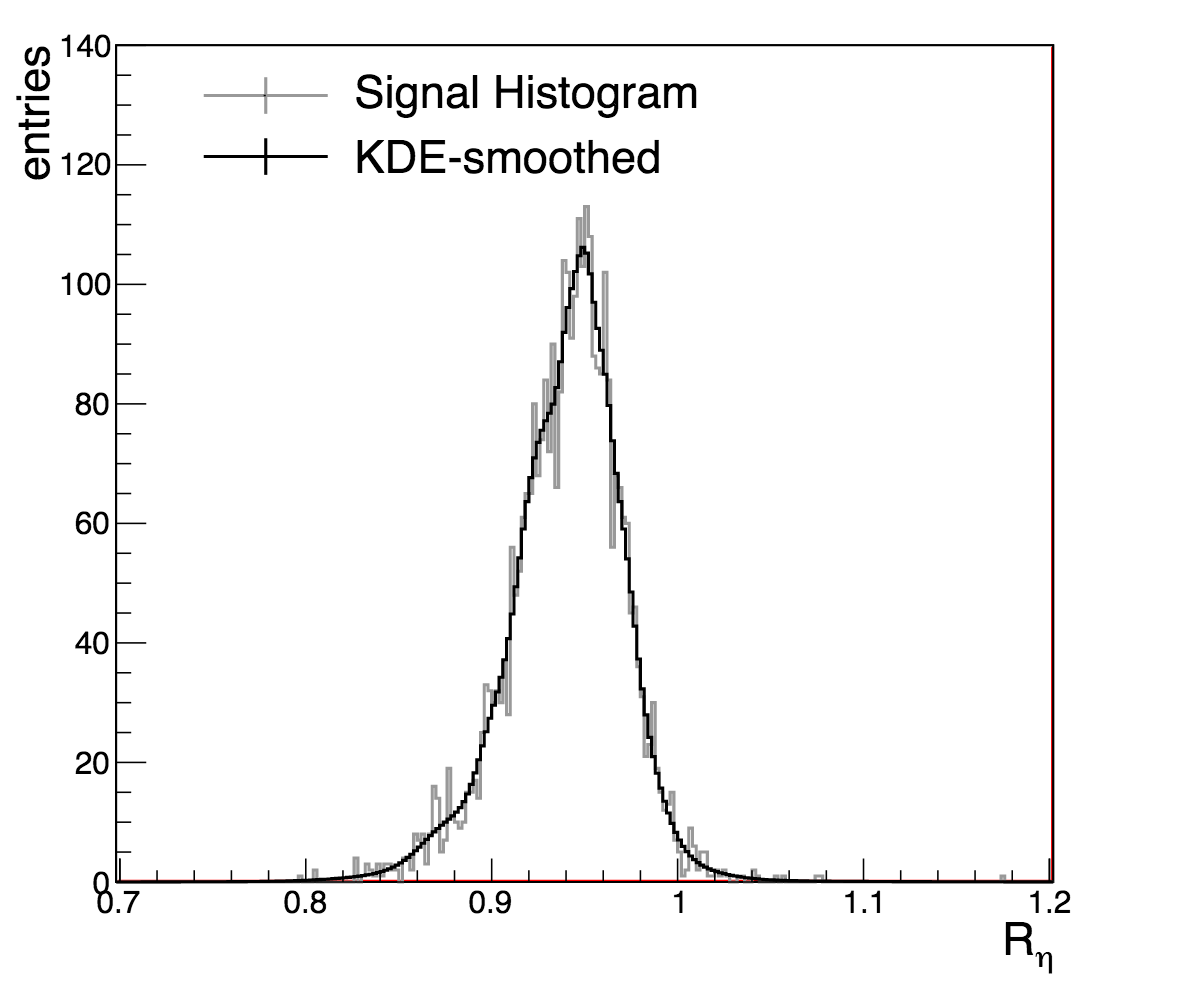
\includegraphics[width=2.5in, height=2.5in]{figures/chapter5/kde_example.pdf}
    \centering
\end{subfigure}
\caption{The KDE Method. Left: a stylized depiction of the standard KDE method (top) and Adaptive KDE method (bottom). Right: an example of a raw variable distribution (grey) and the KDE-smoothed PDF (black).}
\label{fig:kde}
\end{figure}

%% subsec: data vs MC
\subsubsection{Data vs Monte Carlo PDFs}\label{sec:data_vs_mc}
The LH PDFs can be constructed from data or MC events. Using MC allows for the use of truth-matching, where the truth labels described in Chapter 2 are checked to guarantee the objects are or are not electrons. This ensures highly pure signal and background PDFs. However, estimations and imperfect detector modeling in the MC simulation chain results in shape differences between data-driven and MC-driven PDFs, rendering a MC-driven LH less effective when applied to actual data (see Figure \ref{fig:data_v_mc}). These effects can be reduced by adjusting the MC PDFs with data-driven corrections as described in Section \ref{sec:corr_pdfs}, but are not entirely eliminated. On the other hand, data-driven PDFs require additional work to eliminate all contributions from non-desired physics processes and measuring the resulting purity is difficult. In particular, for $J/\psi\rightarrow ee$ PDFs, significant contributions from non-prompt $J/\psi$s (from heavy flavor decays) remain after Tag \& Probe selections and mass cuts. The current method for purifying data-driven $J/\psi\rightarrow ee$ PDFs is described in Section \ref{sec:low_pt_soft}\\

\begin{figure}[hbt!]
\begin{subfigure}
    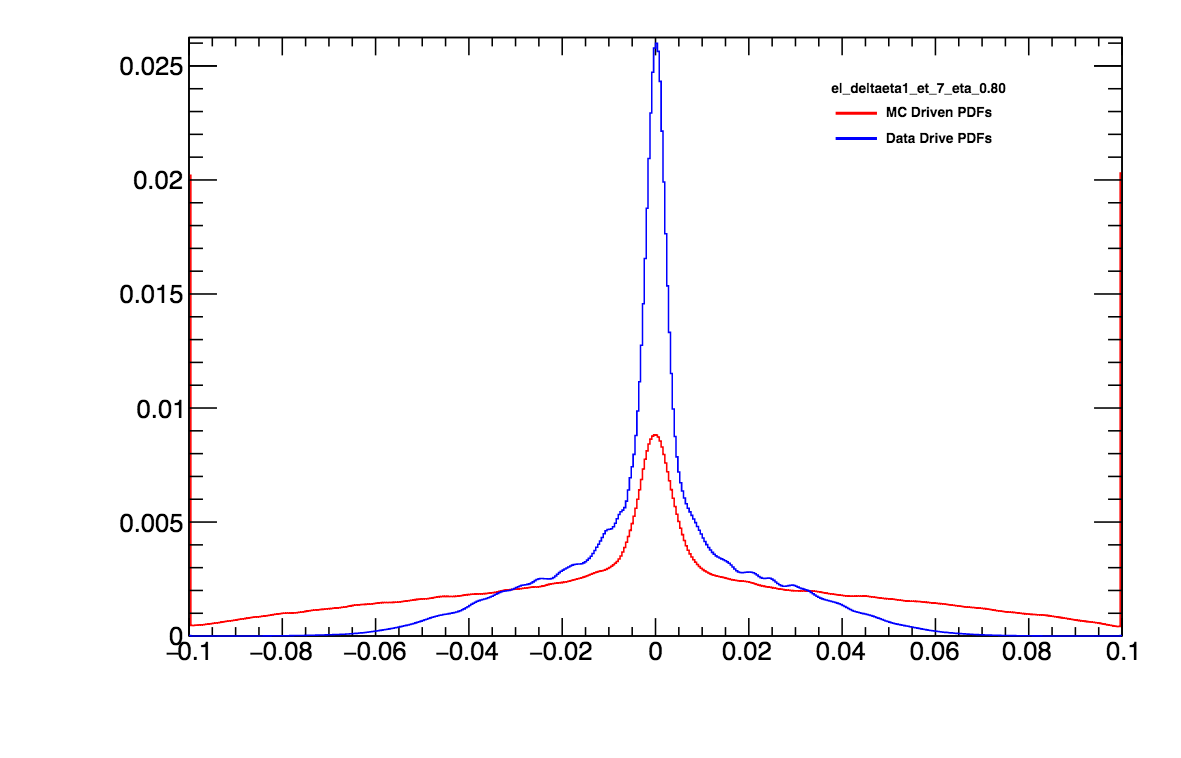
\includegraphics[width=2.5in]{figures/chapter5/data_v_mc_pdf_1.pdf}
    \centering
\end{subfigure}
\begin{subfigure}
    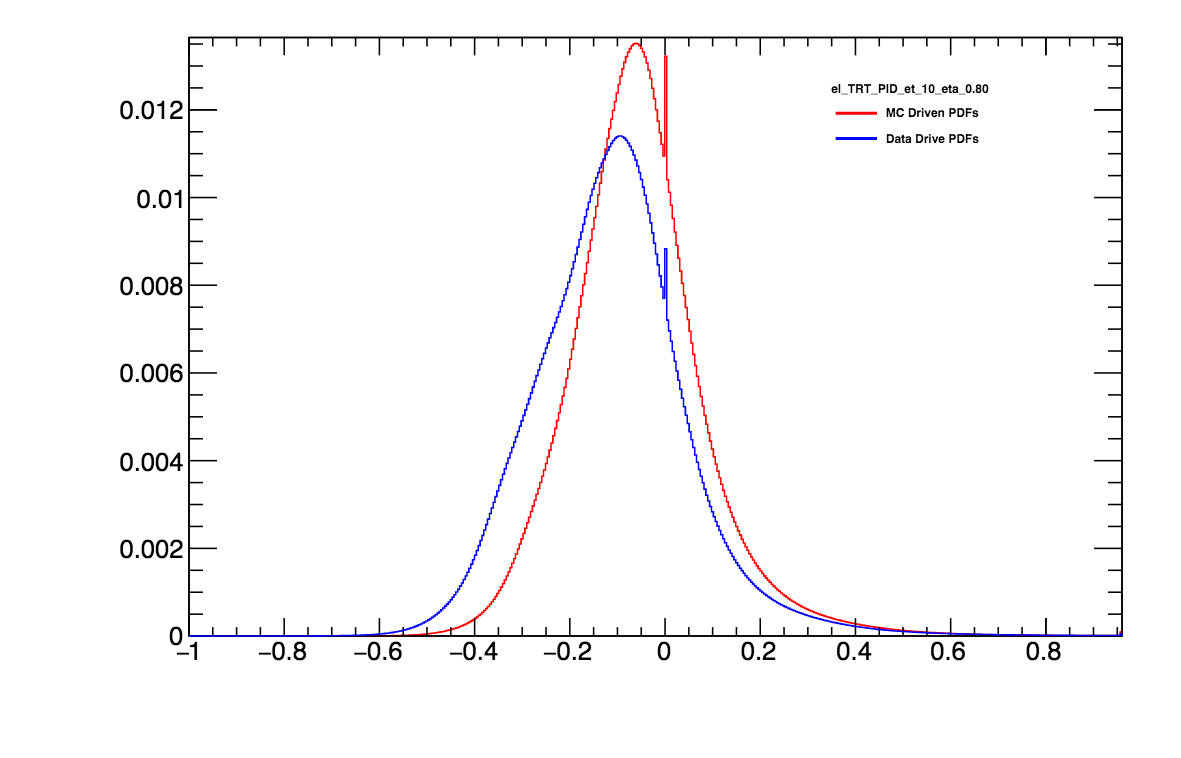
\includegraphics[width=2.5in]{figures/chapter5/data_v_mc_pdf_2.pdf}
    \centering
\end{subfigure}
\caption{Comparisons of data-driven (blue) and MC-based (red) PDFs in the 7 GeV $<p_T<$ 10 GeV and 0.8 $<|\eta|<$ 1.15 bin for two variables. $\Delta\eta_1$ on the left and eProbabilityHT on the right.}
\label{fig:data_v_mc}
\end{figure}

\pagebreak 

In Run 1, data-driven PDFs were used to build the electron ID LH. However, there was no software implemented to construct $J/\psi\rightarrow ee$ PDFs pure enough to build an efficient LH discriminant. Consequently, the $Z\rightarrow ee$ PDFs from the lowest $p_T$ bin with high enough statistics (15-20 GeV) were used for all lower $p_T$ bins. This resulted in reduced electron ID efficiency below 15 GeV. For the first portion of Run 2, MC PDFs were used for the full $p_T$ range of the electron LH. After sufficient Run 2 data was collected and methods for constructing purified $J/\psi\rightarrow ee$ PDFs were developed, a data-driven electron LH ID was introduced and will be used for all full Run 2 analyses. 

\subsubsection{Correcting PDFs}\label{sec:corr_pdfs}
When MC PDFs are used in the electron ID LH they must be corrected to more closely match the distributions seen in data. Most of the first order differences between MC and data PDFs take the form of a constant offset or a width difference (i.e. the Full Width at Half Maximum, FWHM). \\

These differences are corrected by adjusting each electron's PDF entry, $\nu$, to $\nu^*_{MC}=\nu_{MC}-a$ for a constant offset $a$, or $\nu^*_{MC}=(\nu_{MC}-\bar{\nu}_{data,MC})*w$ for width parameter $w$ and mean value $\bar{\nu}_{data,MC}$. Optimal values for $a$ are found by minimizing the $\chi^2$ test statistic, $\chi^2=\sum_{bins}(n_{data}-n_{MC})^2/(\sigma_{data}+\sigma_{MC})$ while the optimal values for $w$ are taken to be the ratio of FWHM between data and MC.\\ 

Corrections are calculated and applied separately for each $\eta$ bin, but do not depend on $p_T$. The corrections derived from signal samples are also applied to background samples. An example of MC PDFs before and after these corrections can be seen in Figure \ref{fig:corr_mc}. These corrections can be applied before or after KDE smoothing as the differences between the results of the two orderings was found to be negligible \cite{id_note}.

\begin{figure}[h]
\begin{subfigure}
    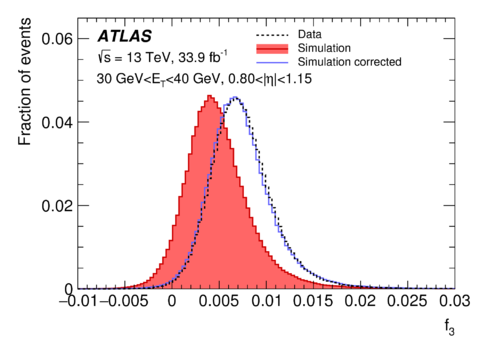
\includegraphics[width=2.5in]{figures/chapter5/corr_mc_1.png}
    \centering
\end{subfigure}
\begin{subfigure}
    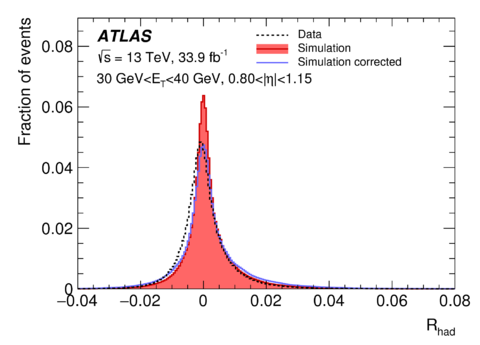
\includegraphics[width=2.5in]{figures/chapter5/corr_mc_2.png}
    \centering
\end{subfigure}
\caption{The $f_3$ (left) and $R_{had}$ (right) PDFs for data (black dashed line) and MC (solid red) in the 30 GeV$<p_T<$40 GeV and 0.8$<|\eta|<$1.15 bin. The MC is shown before (solid red) and after (blue line) corrections have been applied.}
\label{fig:corr_mc}
\end{figure}

%% SECTION: Low PT
\section{Low $p_T$ Electron ID}\label{low_pt_sec}
Electrons with a $p_T$ between 4.5 and 15 GeV are referred to as
``low $p_T$" electrons. These electrons are treated separately from the ``nominal $p_T$" range electrons ($p_T\geq 15$ GeV) because probe electrons from the physics process, $Z\rightarrow ee$, used to build and tune nominal $p_T$ PDFs and LHs has very low statistics below 15 GeV . This leads to increased relative background contamination in the PDFs (as seen in Figure \ref{2012_disc}) and results in decreased ID performance \cite{lh_paper}.\\


\begin{figure}[hb!]
\begin{subfigure}
    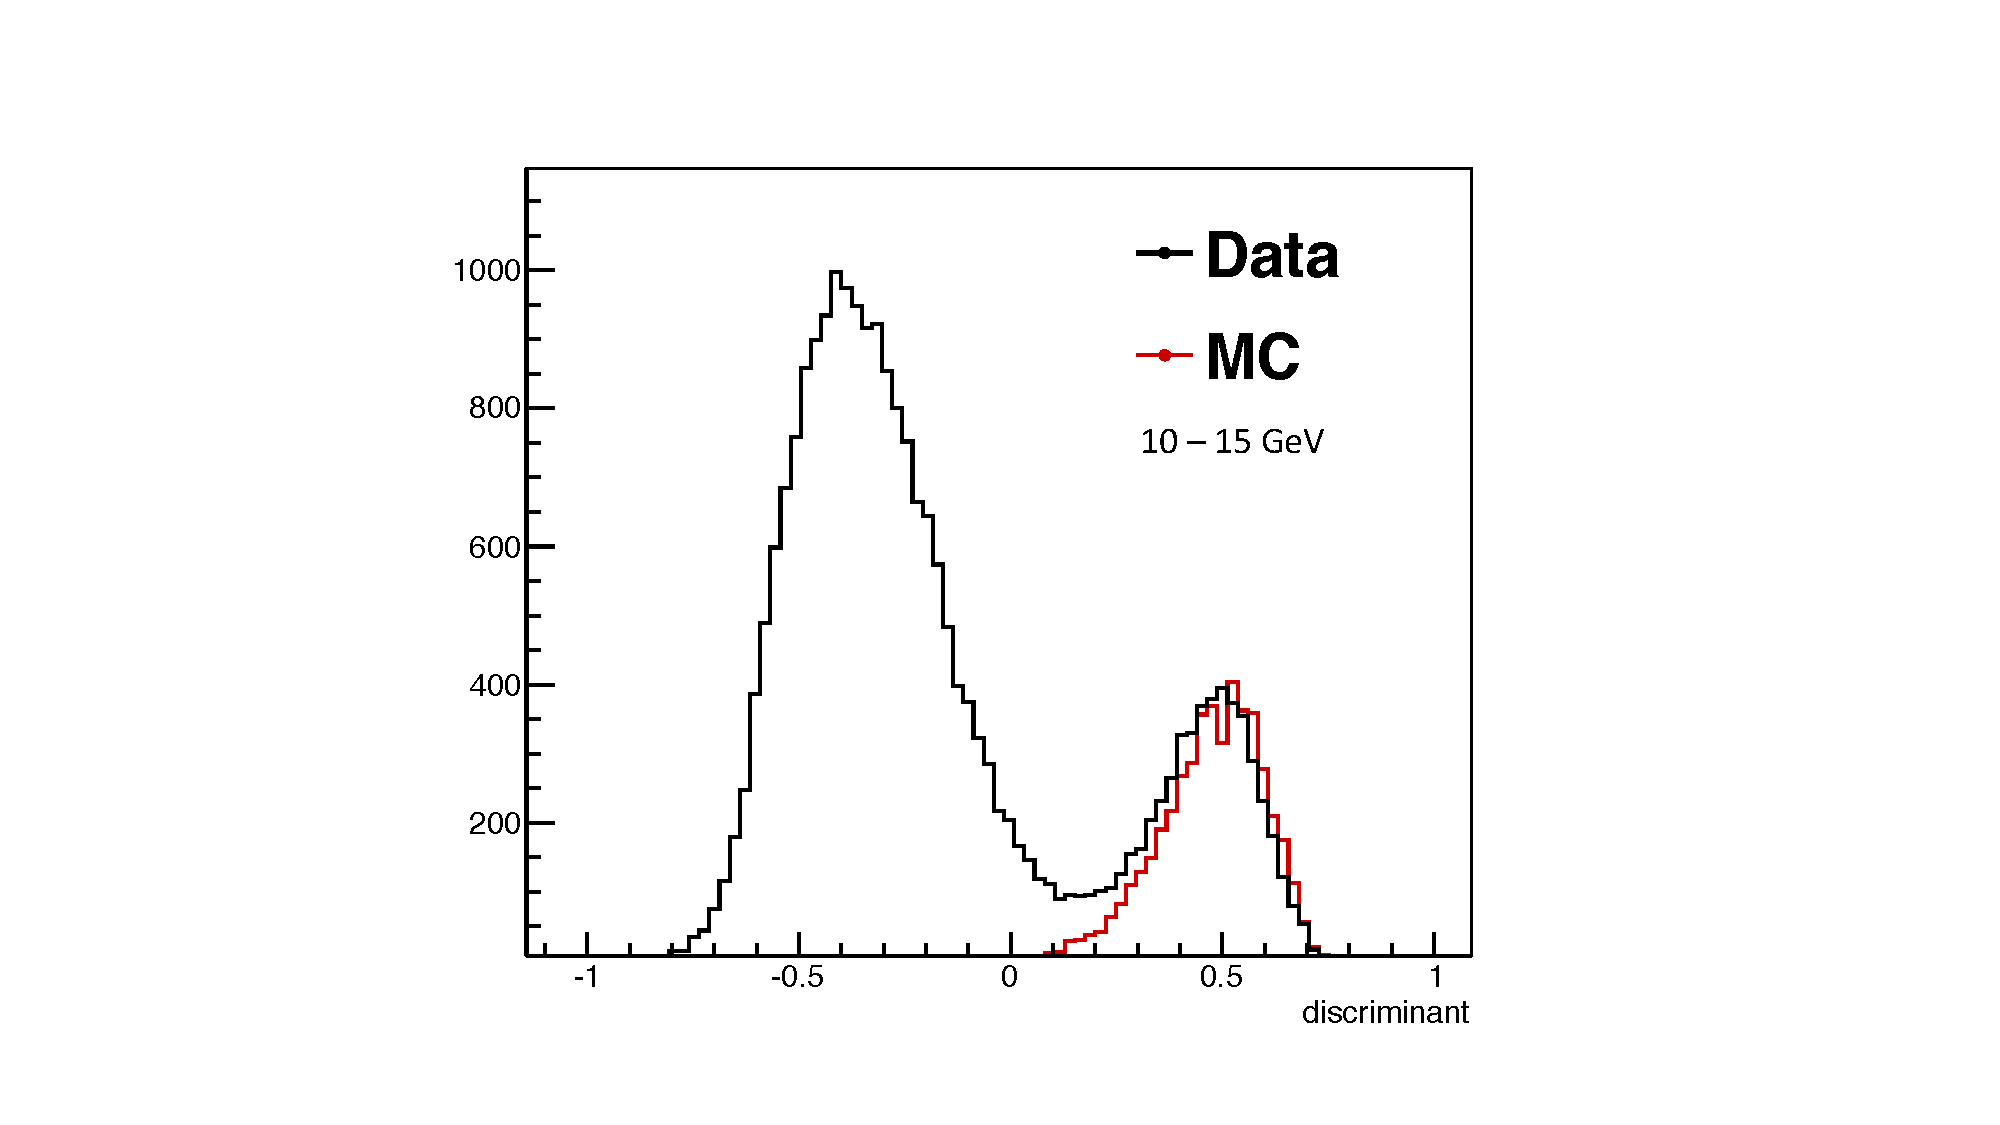
\includegraphics[width=2.5in, height=2.5in]{figures/chapter5/10_15_disc.pdf}
    \centering
\end{subfigure}
\begin{subfigure}
    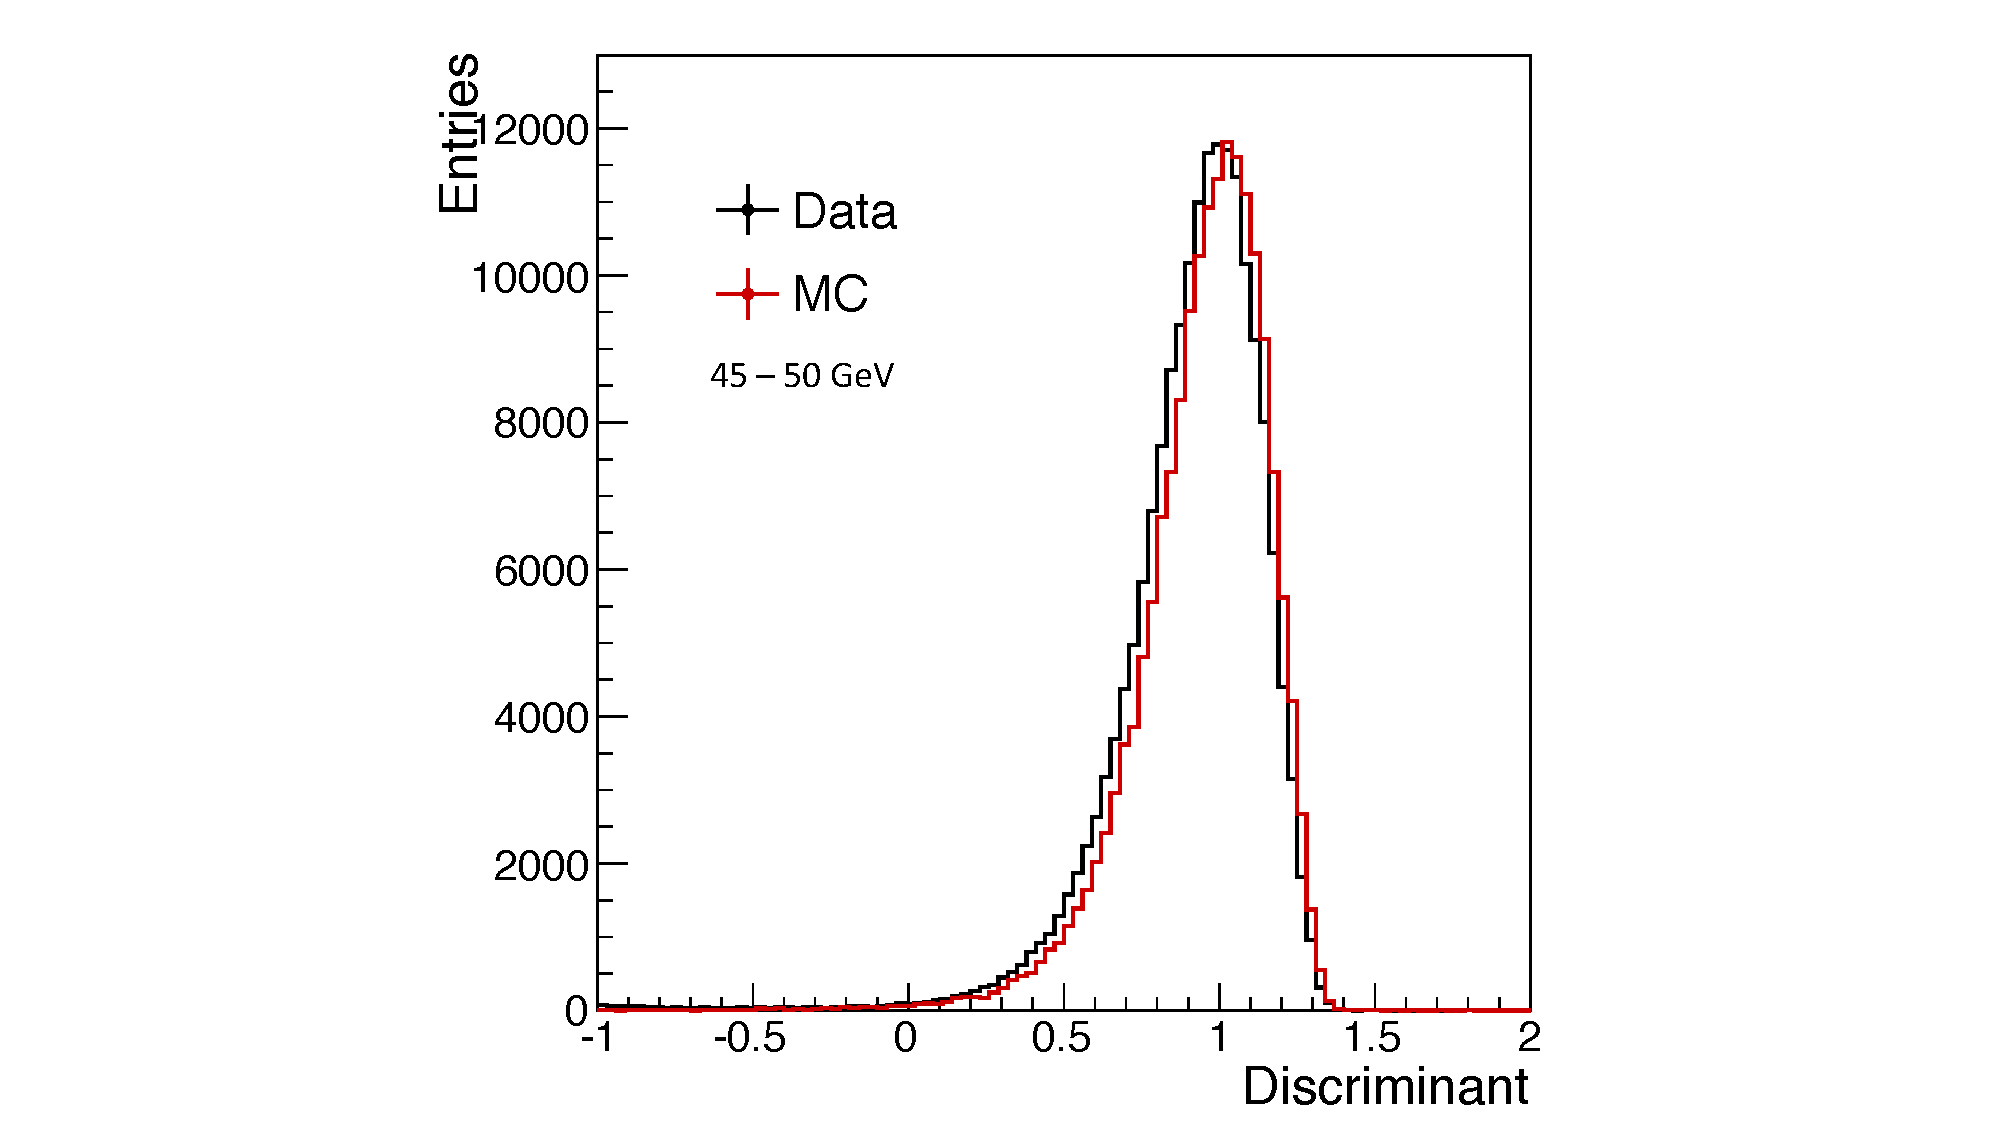
\includegraphics[width=2.5in, height=2.5in]{figures/chapter5/45-50_GeV_disc_2012.pdf}
    \centering
\end{subfigure}
\caption{Left: An example plot of the output discriminant for probes (data and $Z\rightarrow ee$ MC) in the 10 GeV $<p_T<$ 15 GeV and 0.80 $<|\eta|<$ 1.15 bin. The data peak at high discriminant value comes from electrons but the larger peak at low discriminant value is background. Right: the same plot for 40 GeV $<p_T<$ 45 GeV. The fraction of background in the data sample for this $p_T$ range is negligible.}
\label{2012_disc}
\end{figure}

%% SUBSECTION: MOTIVATION
\subsection{Motivation}

Effective identification of low $p_T$ electrons is critical to a variety of ATLAS analyses. One such class of analyses is searches for compressed Supersymmetry which frequently look for event topologies where the supersymmetric particles are produced in association with a colored Initial State Radiation (ISR) jet (see Fig \ref{isr_susy}). If the ISR jet has a high momentum, the recoil of the supersymmetric particles creates a signature of a back-to-back ISR jet and large MET coupled with very soft leptons (as low as 4 GeV) \cite{soft_lep_susy}. Similar signatures are seen in direct Dark Matter production searches where the recoiling object can be a photon\cite{dm_photon} or a hadronic jet \cite{dm_jet}. Finally, low $p_T$ electrons are important to precision measurements of the $H\rightarrow ZZ^*\rightarrow 4l$ decay channel where the off-shell Z boson can be low mass and subsequently decay to soft electrons \cite{h_4l}.

\begin{figure}[hb!]
    \centering
    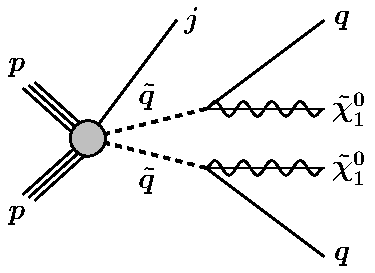
\includegraphics[width=3in]{figures/chapter5/isr_susy.pdf}
    \caption{Production of a pair of squarks with an ISR jet\cite{dm_jet}.}
    \label{isr_susy}
\end{figure}


%% SUBSECTION: SOFTWARE
\subsection{Software Development}\label{sec:low_pt_soft}
The technical capability to construct data-driven low $p_T$ PDFs from $J/\psi\rightarrow ee$ events was developed in Run 2. The PDFs are constructed using a Tag \& Probe selection and events are collected using secondary di-electron trigger. Tag electrons are required to pass the Tight Operating Point and have a $p_T$ of at least 4.5 GeV (reduced from 7 GeV in Run 1 in order to access softer electrons). The probe electron must form an invariant mass with the tag within a 0.5 GeV window of the $J/\psi$ mass (3.8 - 4.3 GeV) and the tag and probe must be separated by $\Delta R> 0.1$ to avoid overlap between the two objects. \\

\begin{figure}[hbt!]
    \centering
    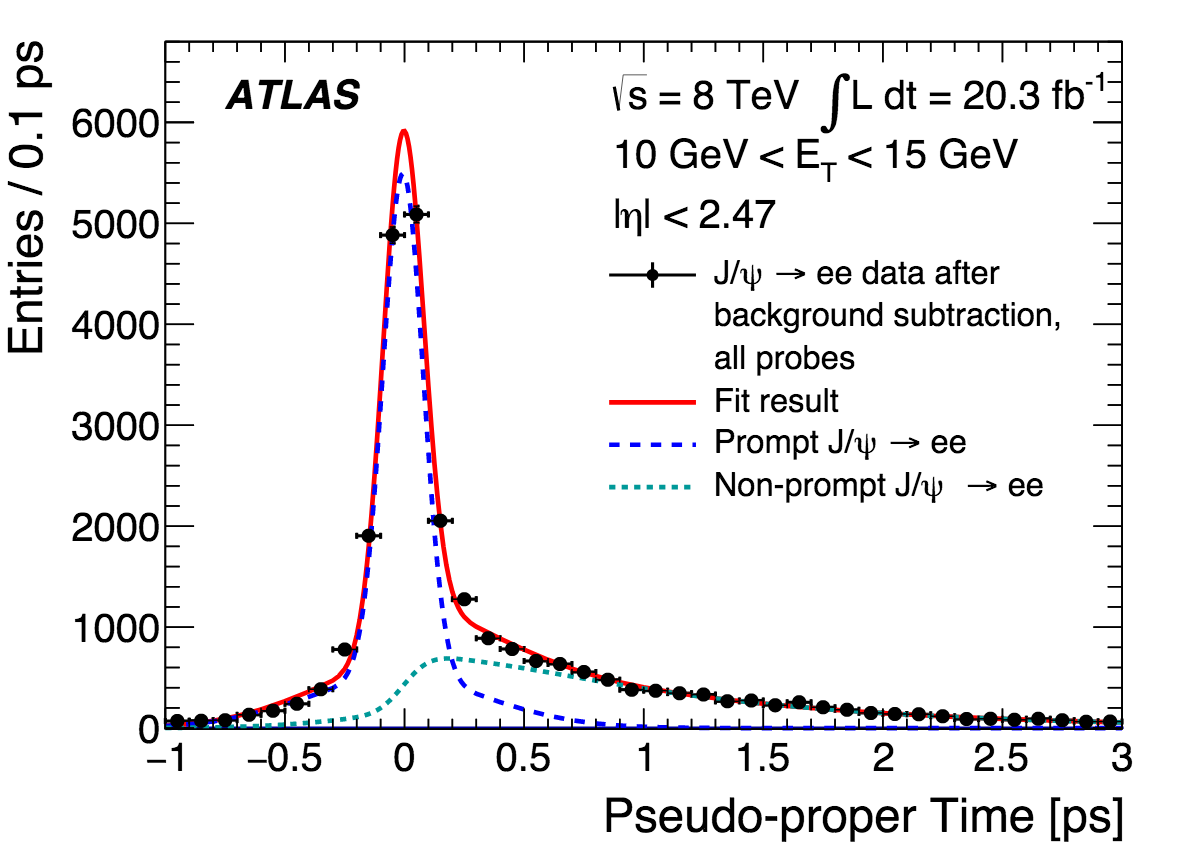
\includegraphics[width=4in]{figures/chapter5/tau_probes.pdf}
    \caption{Pseudo-proper time for all probe electron candidates. The prompt signal component is shown by the dashed blue line and the non-prompt signal component is shown by the light blue dashed line.}
    \label{fig:tau_probes}
\end{figure}

The main challenge in constructing data-driven $J/\psi\rightarrow ee$ PDFs is the presence of non-prompt $J/\psi$ candidates (mainly from b-quark decays) after the selections described above are applied. To remove these contributions, a cut is placed on the pseudo-proper time of the $J/\psi$ candidates. Pseudo-proper time, $\tau$, is defined as $\tau=(L_{xy}*m^{J/\psi})/(p_T^{J/\psi})$ where $L_{xy}$ is the distance from the primary event vertex to the $J/\psi$ vertex. An example $\tau$ distribution for probe electrons can be seen in Figure \ref{fig:tau_probes}. For Run 2, probe electrons are required to have a pseudo-proper time -1 ps $<\tau<$ 0.2 ps and the dielectron invariant mass distribution for signal and background using this cut is shown in Figure \ref{fig:tau_cuts}.

\begin{figure}[hbt!]
    \centering
    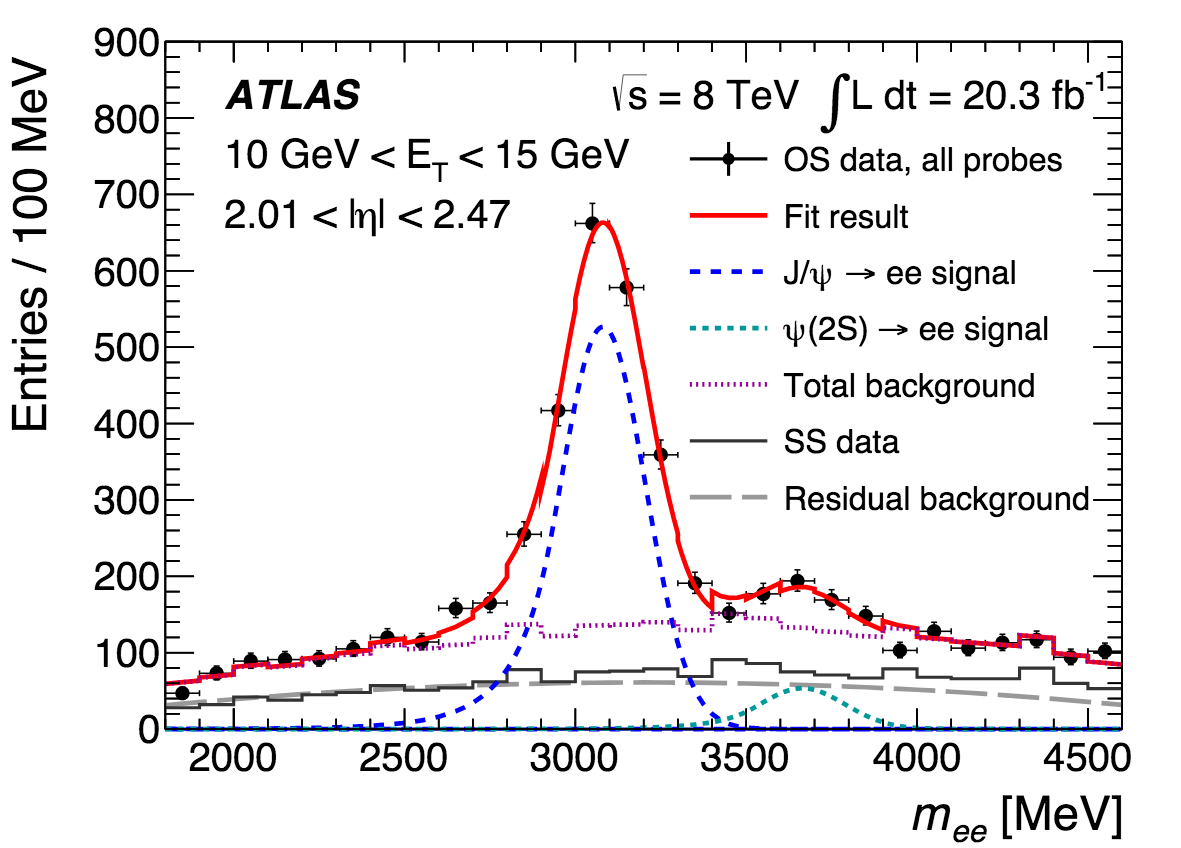
\includegraphics[width=4in]{figures/chapter5/before_tau_cut.pdf}
    \caption{Dielectron invariant-mass fit for all probe electron candidates. The pseudo-proper time is required to be $-1$ ps $ < \tau < 0.2$ ps. Dots with error bars represent the opposite-sign (OS) pairs for data, the fitted $J/\psi$ signal is shown by the dashed blue and the $\psi$(2S) by the dashed light blue lines. The sum of the background contributions is depicted as a purple dotted line.}
    \label{fig:tau_cuts}
\end{figure}

%% SUBSECTION: Variable OPT
\subsection{Variable Optimization}
Despite transitioning to data-driven $J/\psi\rightarrow ee$ PDFs for the low $p_T$ electron ID, the ID efficiency remains lower in this region (Figure \ref{fig:mc_data_eff}). This is likely because this region was not specifically optimized in Run 1, and the same variables chosen for nominal $p_T$ are used at low $p_T$ with no further study. \\

\begin{figure}[hbt!]
    \centering
    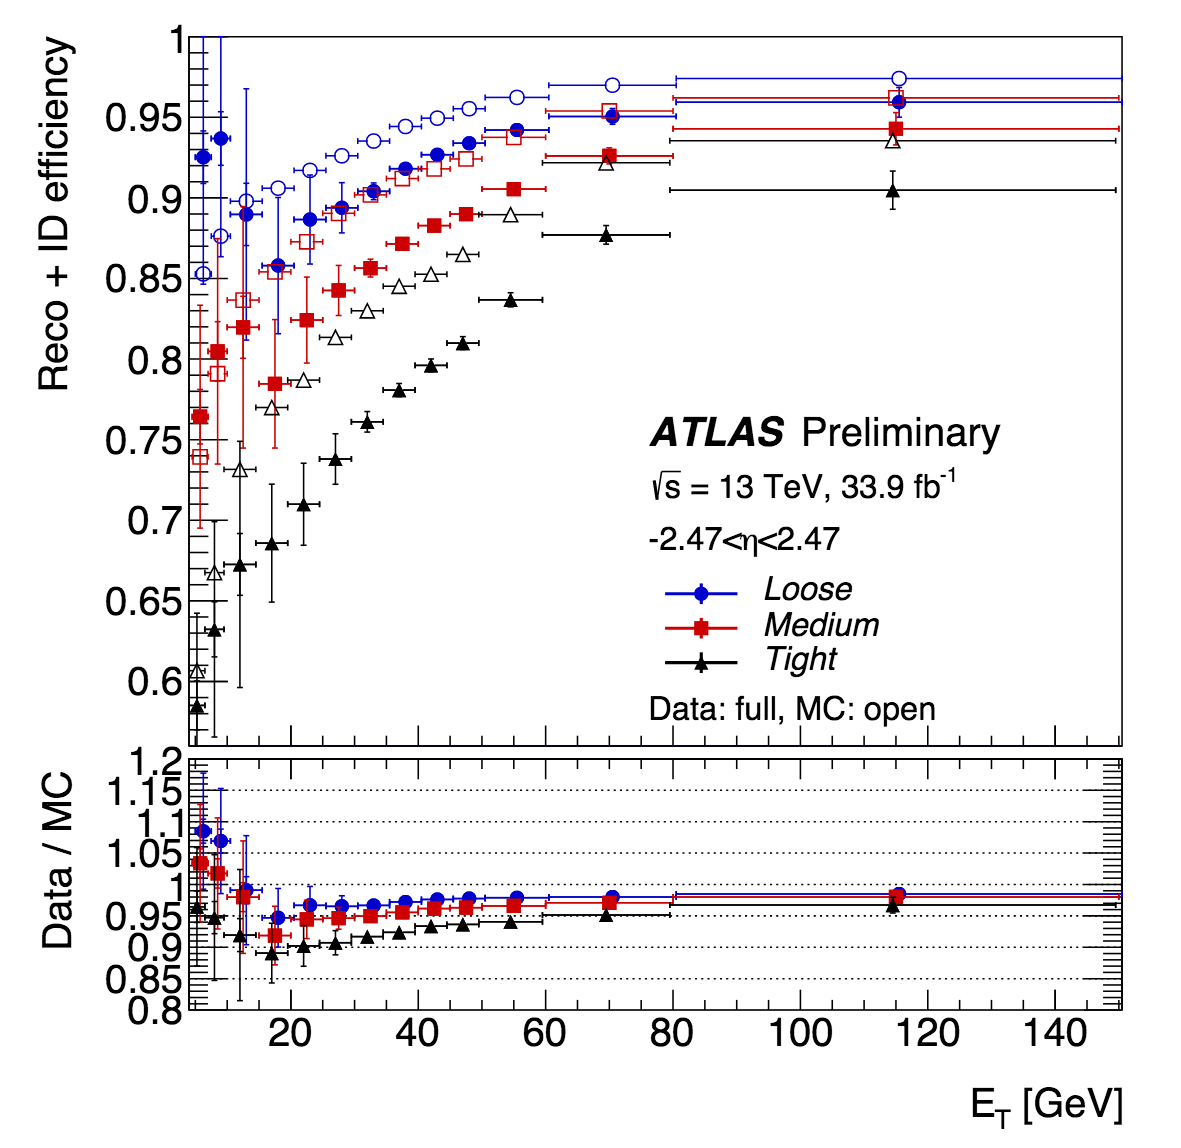
\includegraphics[width=4in]{figures/chapter5/mc_data_eff.pdf}
    \caption{Electron reconstruction and identification efficiencies as a function of transverse energy $E_T$, integrated over the full pseudo-rapidity range.}
    \label{fig:mc_data_eff}
\end{figure}

An ``n-1" LH study was conducted to determine if all LH variables remain efficient in the low $p_T$ range. In this study a set of nearly identical LH operating points were constructed, with the only difference being that each LH removes just one variable from the nominal collection of discriminating variables. The performance of these alternative LH operating points can then be compared to the nominal LH performance by examining the receiver operating characteristic (ROC) curve (Figure \ref{fig:n-1_stud}).  If a given ROC curve is higher than the nominal ROC curve (dotted black curve), then the identification performance for this alternative operating point is better than the nominal operating point, and thus it may be beneficial to remove that particular variable. Several variables including $f_1$ (hot pink line), $f_3$ (olive green line), $w_{\eta 2}$ (black solid line), and $\Delta\phi_{res}$ (aqua blue line) consistently improved performance when removed across most low $p_T$ and $\eta$ bins studied, and could be removed from future iterations of the low $p_T$ LH.\\

\begin{figure}[h]
    \centering
    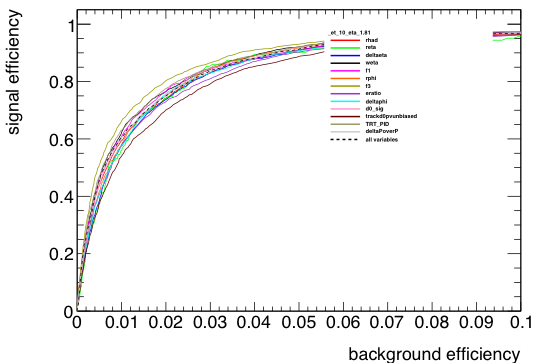
\includegraphics[width=5in]{figures/chapter5/n-1_studies.png}
    \caption{n-1 LH ROC curves. The nominal LH with all variables included is the dashed black line.}
    \label{fig:n-1_stud}
\end{figure}

In addition to optimizing the variables already used in the low $p_T$ region, several new variables are also being studied to further improve low $p_T$ electron ID efficiency. These variables are: 
\begin{itemize}
    \item charge*$d_0$: this would be used in place of the current transverse impact parameter variable $d_0$.
    \item $\Delta$(curvature)/error(curvature): curvature is defined as $1/p_T$ and is well measured at low $p_T$. This variable is sensitive to the amount of energy lost due to bremmstrahlung radiation, which is particularly important in the low $p_T$ region. This variable is a possible replacement for $\Delta p/p$ which is better measured at higher $p_T$.
    \item $\Delta(\Delta\phi)=\Delta\phi_{LM}-\Delta\phi_{FM}$: this variable measures the change in the track-calorimeter match variable $\Delta\phi$ between its value in the first and last layers of the calorimeter. This variable may be useful for identifying converted photons.
\end{itemize}
Comparisons of the PDF shapes of signal and background for these variables can be seen in Figure \ref{fig:new_lowpt_vars}. There are clear shape differences in both $\Delta$(curvature)/error(curvature) and $\Delta(\Delta\phi)$, indicating these variables would likely improve the signal selection efficiency of the low $p_T$ LH. 

\begin{figure}[hbt!]
\centering
\begin{subfigure}
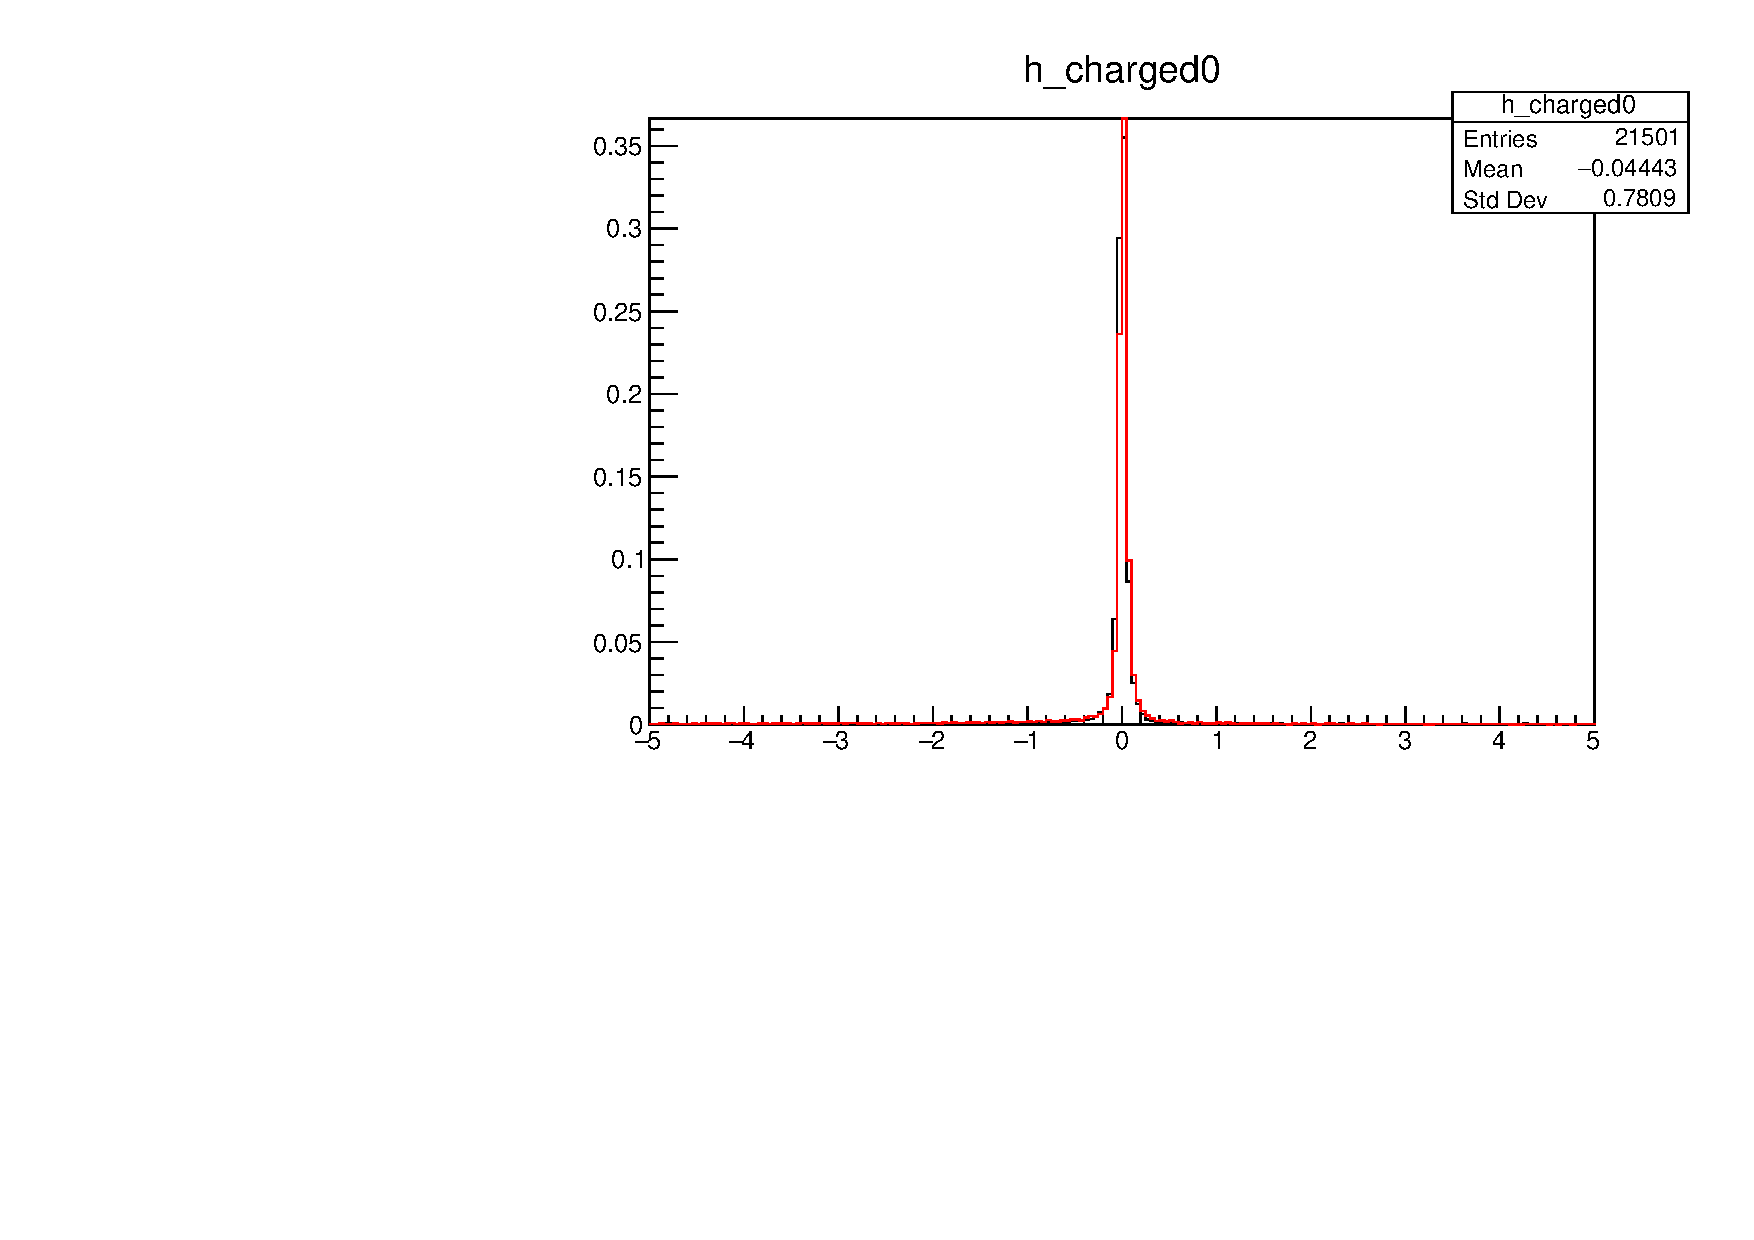
\includegraphics[height=2.5in, angle=270]{figures/chapter5/h_charged0.pdf}
\end{subfigure}
\begin{subfigure}
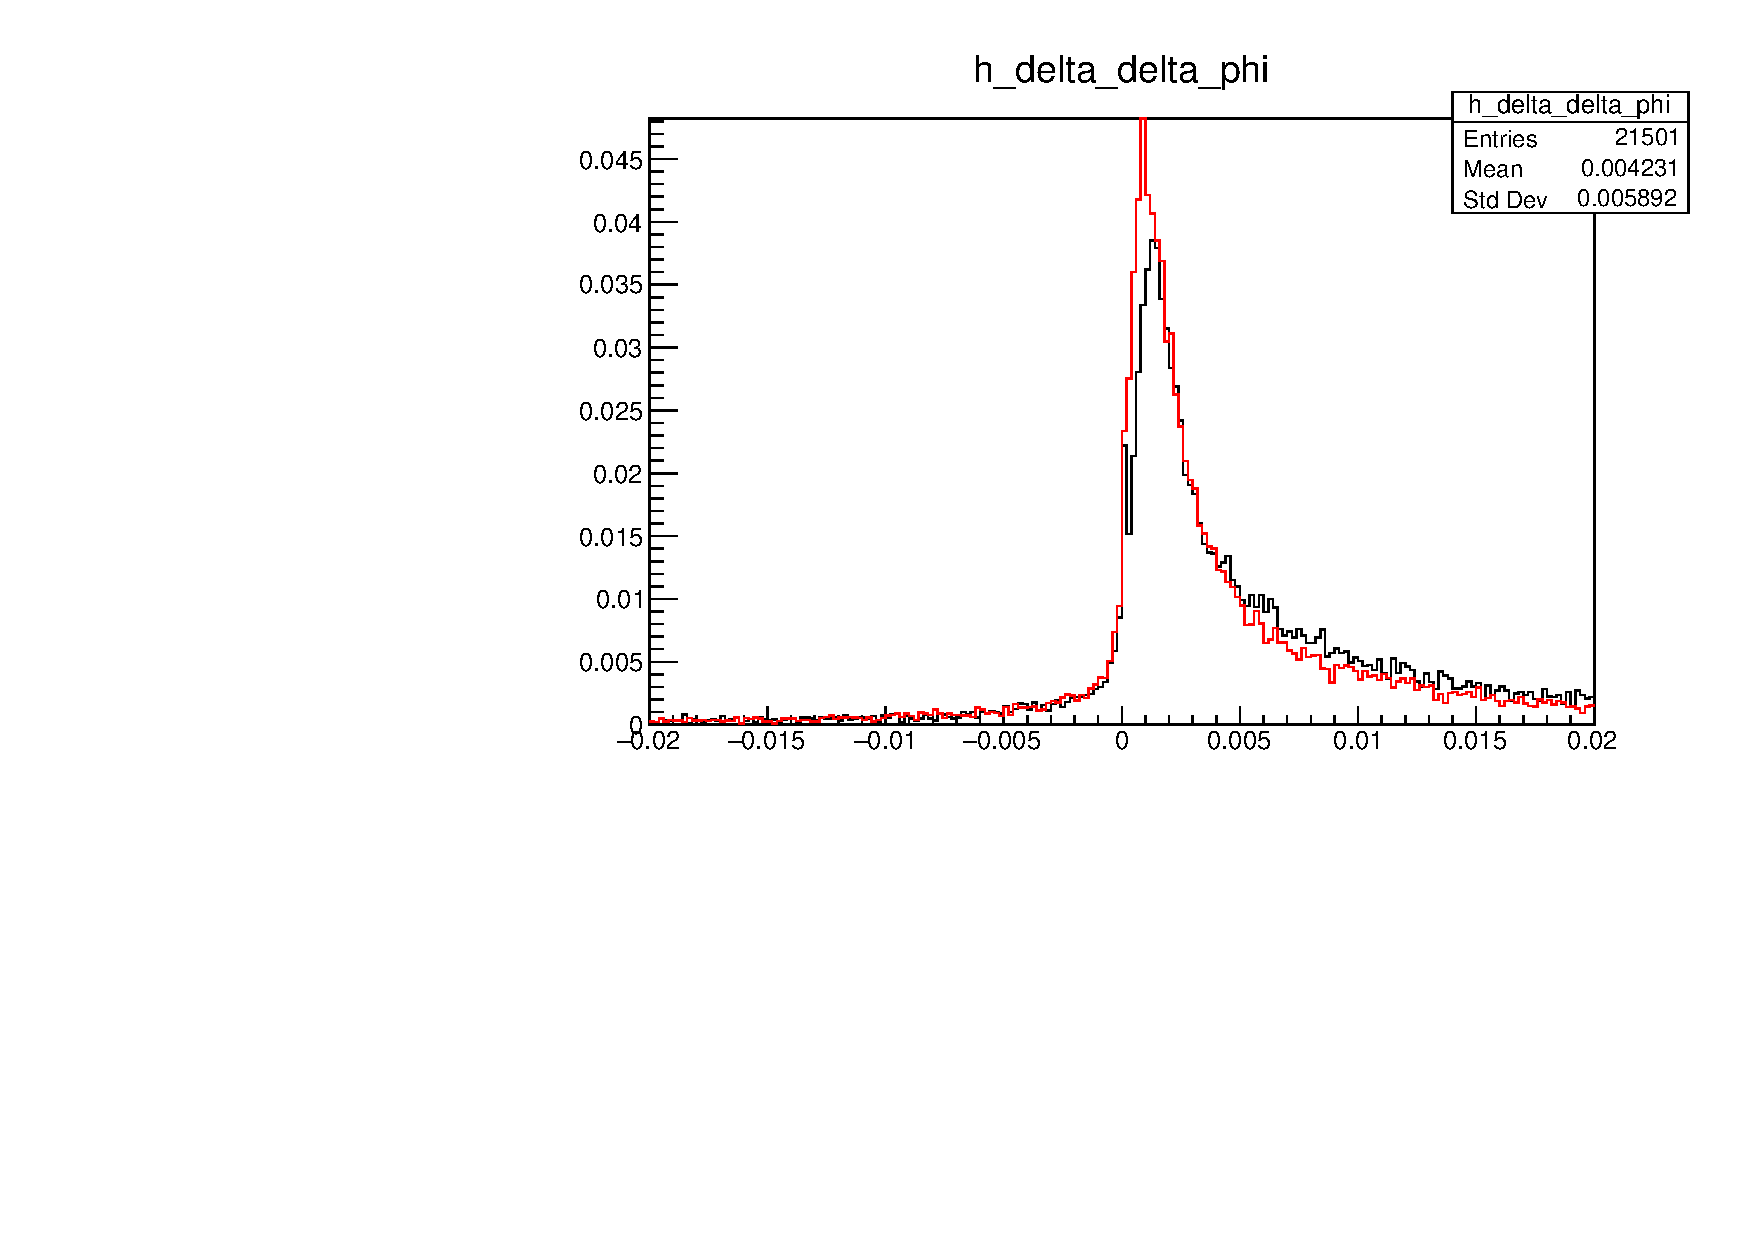
\includegraphics[height=2.5in, angle=270]{figures/chapter5/h_delta_delta_phi.pdf}
\end{subfigure}
\begin{subfigure}
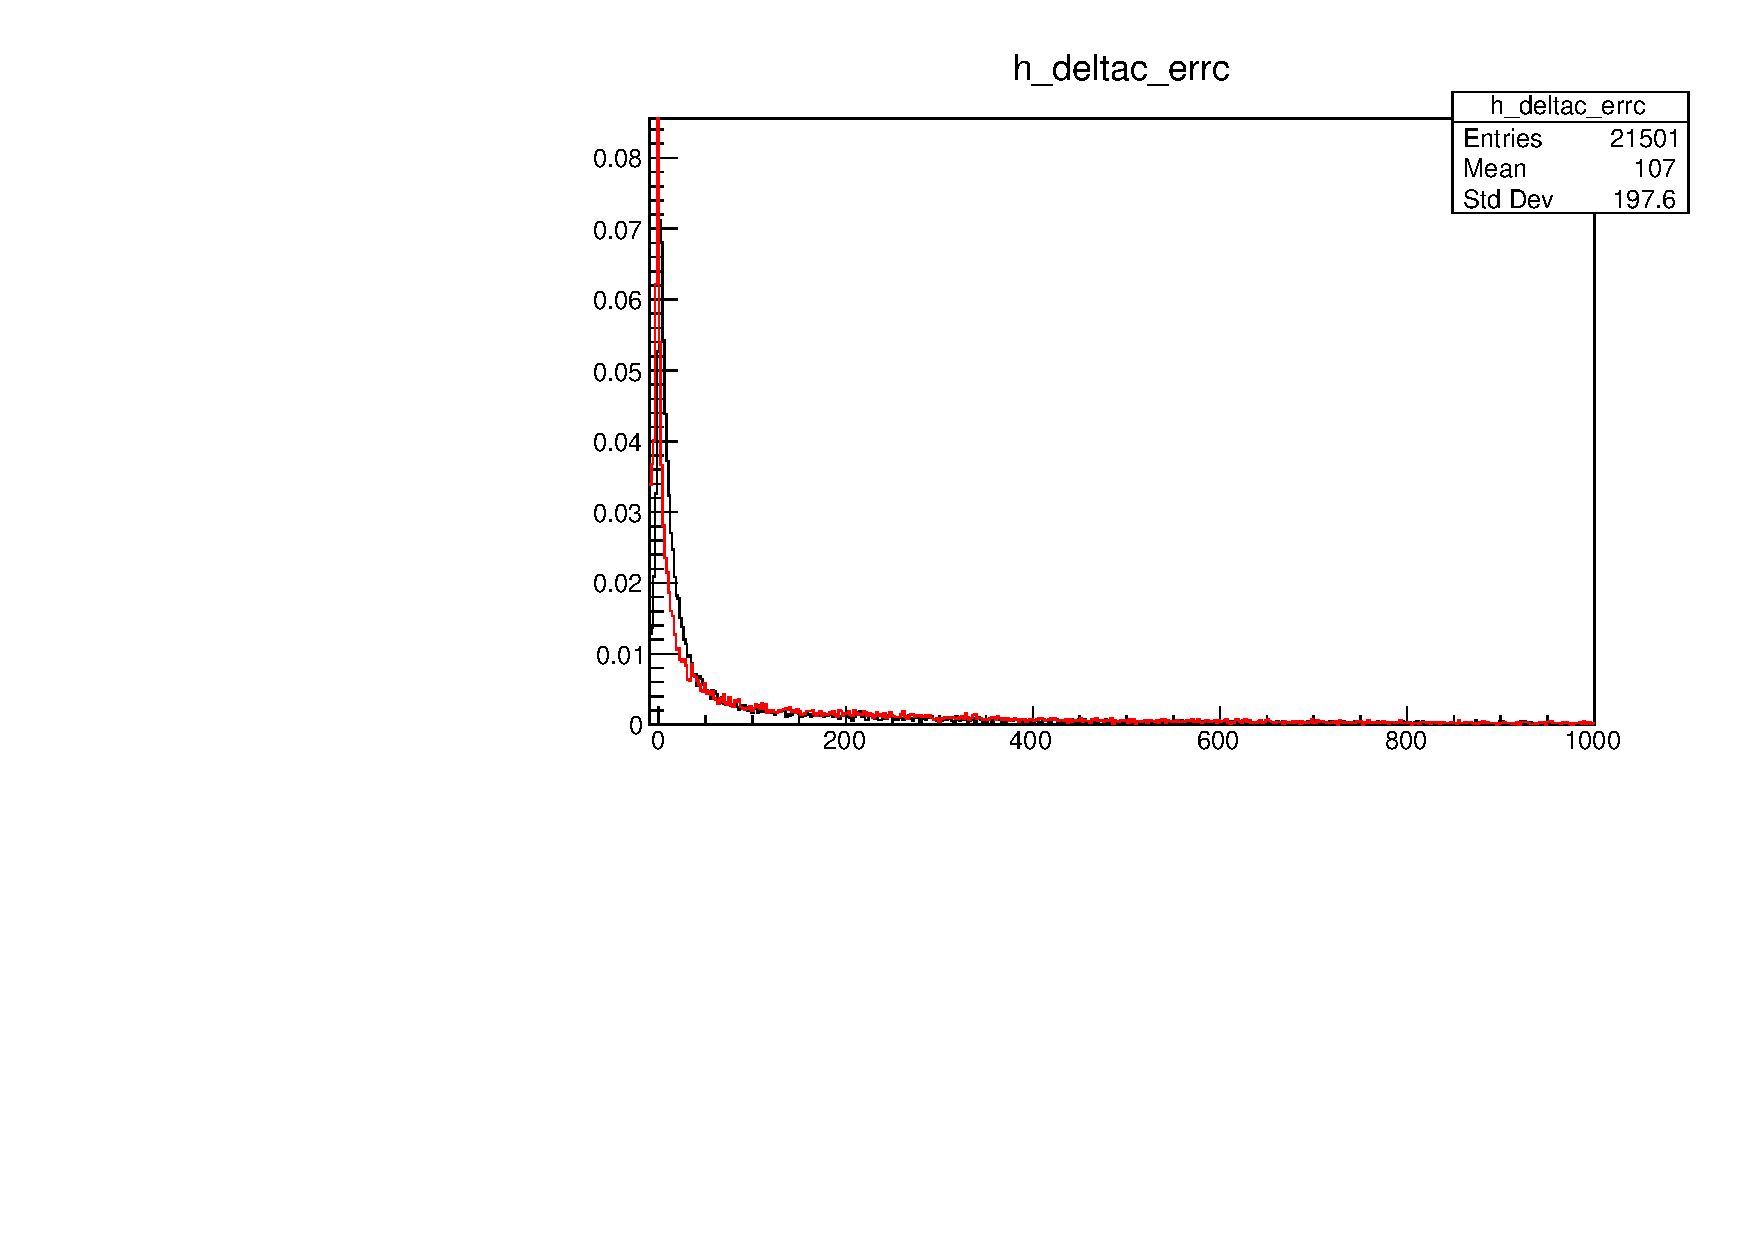
\includegraphics[height=2.5in, angle=270]{figures/chapter5/h_deltac_errc.pdf}
\end{subfigure}
\caption{Comparisons of signal (red) and background (black) PDF shapes for new low $p_T$ variables in the 4.5 GeV $<p_T<$ 7 GeV and 1.81 $<|\eta|<$ 2.01 bin. Top left: charge*$d_0$, top right: $\Delta(\Delta(\phi))$, bottom: $\Delta$(curvature)/error(curvature)}
\label{fig:new_lowpt_vars}
\end{figure}

%%% SECTION: ML
\section{Machine Learning and Electron ID\label{ml_id}}
CNN-driven particle ID using images formed from the hadronic calorimeter has been quite successful (Chapter 4). This technique is currently being studied for application to electron and photon ID in the LAr EM calorimeter.\\

The creation of electron images in the EM calorimeter is more difficult than forming images in the hadronic calorimeter because the detector granularity varies substantially between layers and between the barrel and endcap regions (Chapter 2). A data set of over 2 million events and corresponding images is supported by the ATLAS E/Gamma Working Group. In order to preserve the most information possible, the data-set for these studies contains different granularity images for each layer of the EM calorimeter. The images are formed by first taking all cells in a $7\times 11$ window of the second calorimeter layer (ECAL2) centered on the highest energy cell in the electron ROI. All cells in the other three layers that overlap with this window are included in the image for that layer. A sample image is shown in Figure \ref{fig:elec_imgs}. As is done in many of the jet image applications, initial studies are restricted to the barrel region of the detector. In cases where the ECAL2 $7\times11$ window extends beyond the barrel region the non-barrel pixels are set to zero.\\

\begin{figure}[htb!]
    \centering
    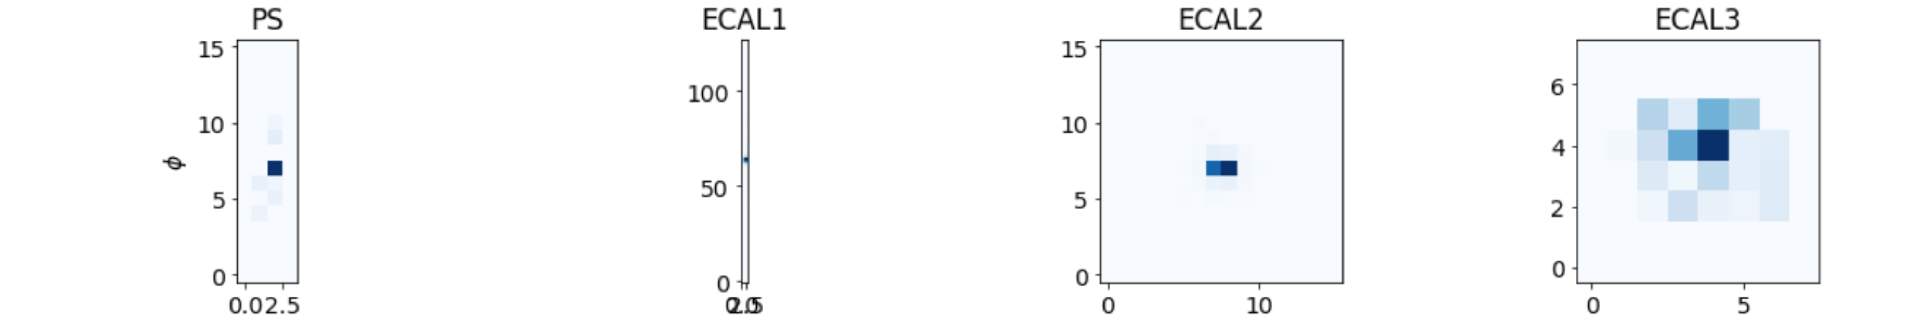
\includegraphics[width=6in]{figures/chapter5/regular_electron_imgs.png}
    \caption{A sample electron image for each of the four EM calorimeter layers.}
    \label{fig:elec_imgs}
\end{figure}

With this method of image construction the CNN architecture design must account for the different layer granularities. For initial studies, the images were all up-sampled to a common granularity of $128\times128$ as shown in Figure \ref{fig:upsamp_elec_imgs} using a Keras 2D upsampling convolutional layer \cite{keras}. The four images are then concatenated into a $128\times128\time4$ stack and processed through a convolutional layer, ReLu activation layer, and a maxpooling layer. The processed images are then flattened and concatenated with additional scalar features of the particle including charge, $\eta$, $\phi$, and TRTPID. This vector is then input into two fully connected NNs, one of which predicts a classification value (truth is 1 for signal and 0 for backgrounds) and one of which predicts a scale factor to calibrate the particle energy. The network was entirely constructed in Keras with a TensorFlow \cite{tensorflow} back end and the full architecture is shown in Figure \ref{fig:elec_cnn}.\\ 

\pagebreak

\begin{figure}[htb!]
    \centering
    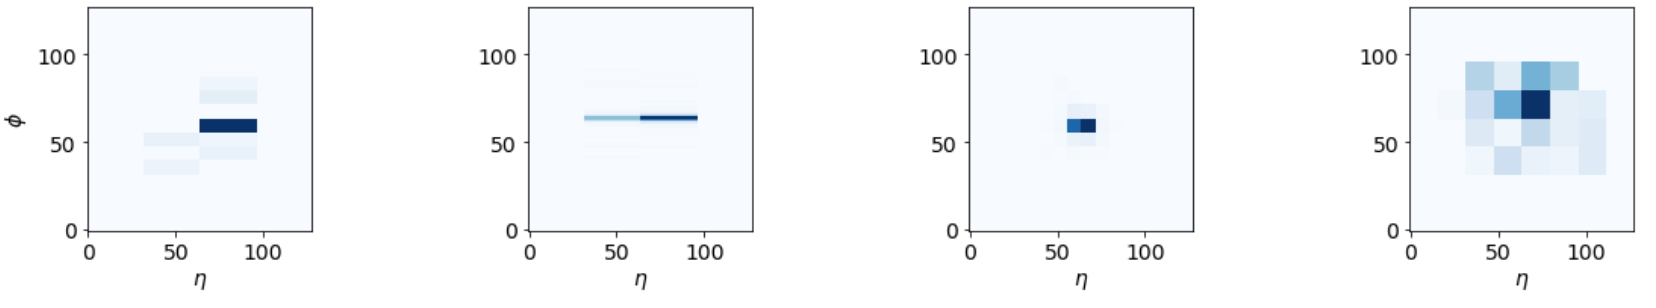
\includegraphics[width=5.5in]{figures/chapter5/upsamp_elec_imgs.png}
    \caption{The same electron image from Figure \ref{fig:elec_imgs} after being up-sampled to a uniform granularity of $128\times128$.}
    \label{fig:upsamp_elec_imgs}
\end{figure}

\begin{figure}[htb!]
    \centering
    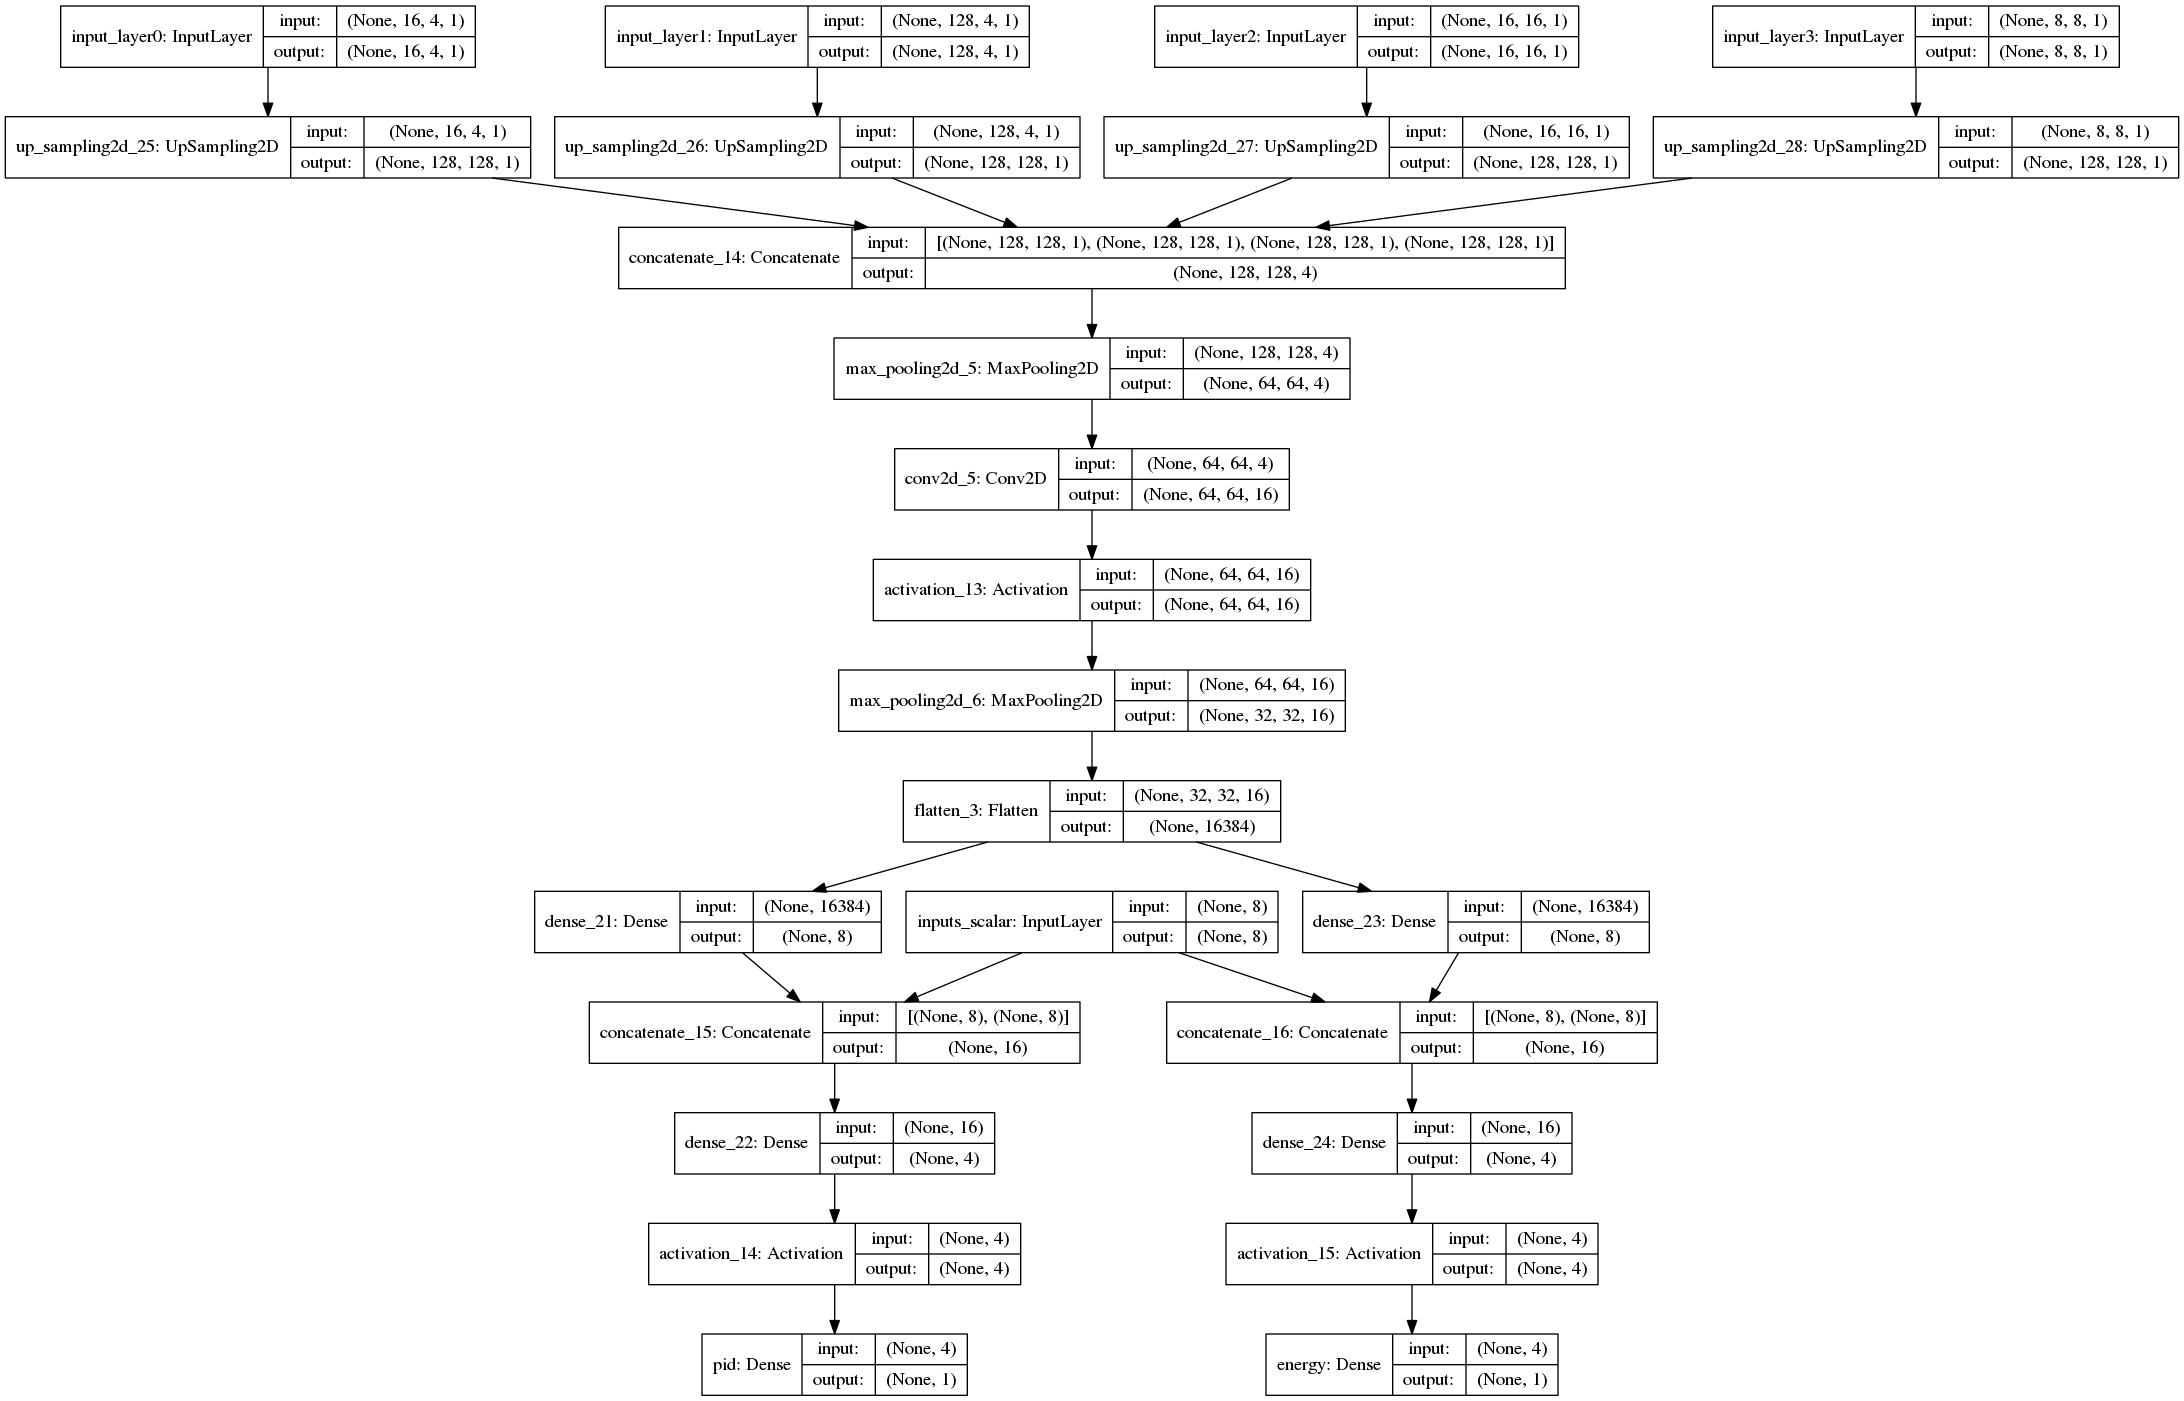
\includegraphics[width=5.5in]{figures/chapter5/electron_cnn_network.png}
    \caption{Network architecture for image-based electron ID and calibration.}
    \label{fig:elec_cnn}
\end{figure}

The network was trained using 1 million signal (prompt electron) samples and 100,000 background ($2\rightarrow2$ QCD processes) samples where 20\% was held-out for the test-set and 20\% for the validation set. The training process used standard backpropagation with a binary cross-entropy loss function. Results of the two tasks are shown in Figures \ref{fig:elec_id_cnn} and \ref{fig:elec_calib_cnn}; the classification task achieves excellent signal-background separation and the calibration task actually outperforms the current ATLAS E/Gamma algorithm \cite{egam_calib}. 

\begin{figure}[htb!]
    \centering
    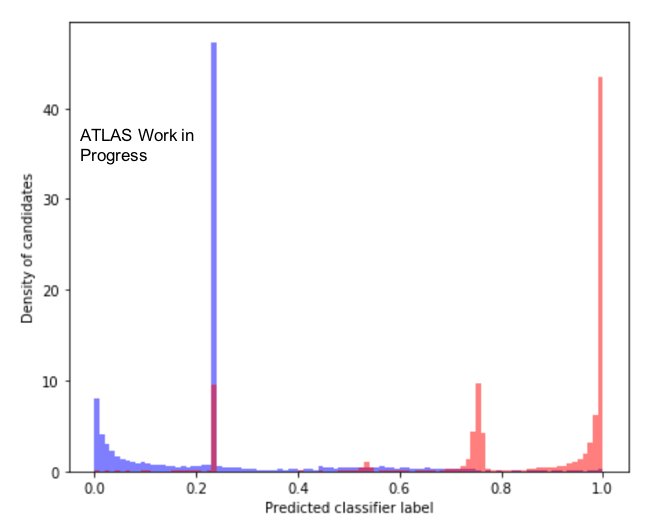
\includegraphics[width=3.5in]{figures/chapter5/elec_id_cnn_plot.png}
    \caption{Classifier output of  the image-based electron ID CNN for signal (red) and background (blue).}
    \label{fig:elec_id_cnn}
\end{figure}

\begin{figure}[htb!]
    \centering
    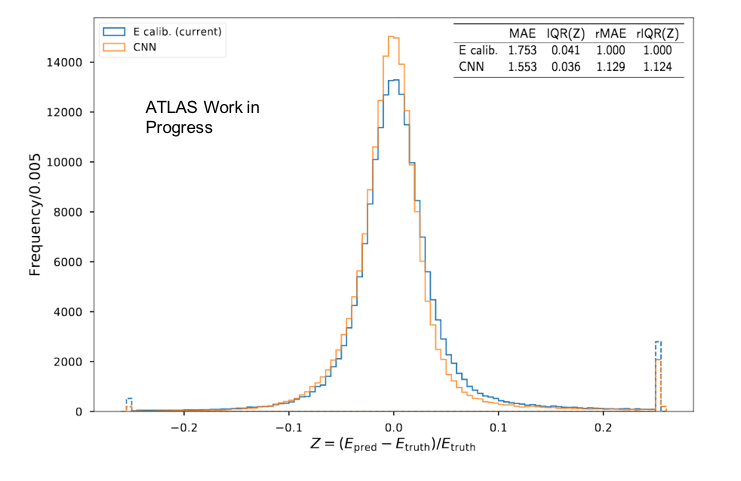
\includegraphics[width=3.5in]{figures/chapter5/elec_calib_cnn_plot.png}
    \caption{Normalized difference between predicted particle energy and truth particle energy for the imaged-based calibration CNN (orange) and the standard ATLAS electron calibration algorithm (blue).}
    \label{fig:elec_calib_cnn}
\end{figure}

\subsection{Future Studies}
This area of research is on-going and there are several techniques being studied to improve upon the performance described above. For instance, there are other possible ways of addressing the granularity mis-match such as applying a separate convolution to each layer image and concatenating them just before the task networks or up-sampling and applying a 3D convolution (Figure \ref{fig:3d_conv}) that would allow the network to learn relationships between the EM calorimeter layers. Additionally, track information can be included in either by including it in the scalar feature concatenation or by creating track images using the Inner Detector outputs.\\

\begin{figure}[htb!]
    \centering
    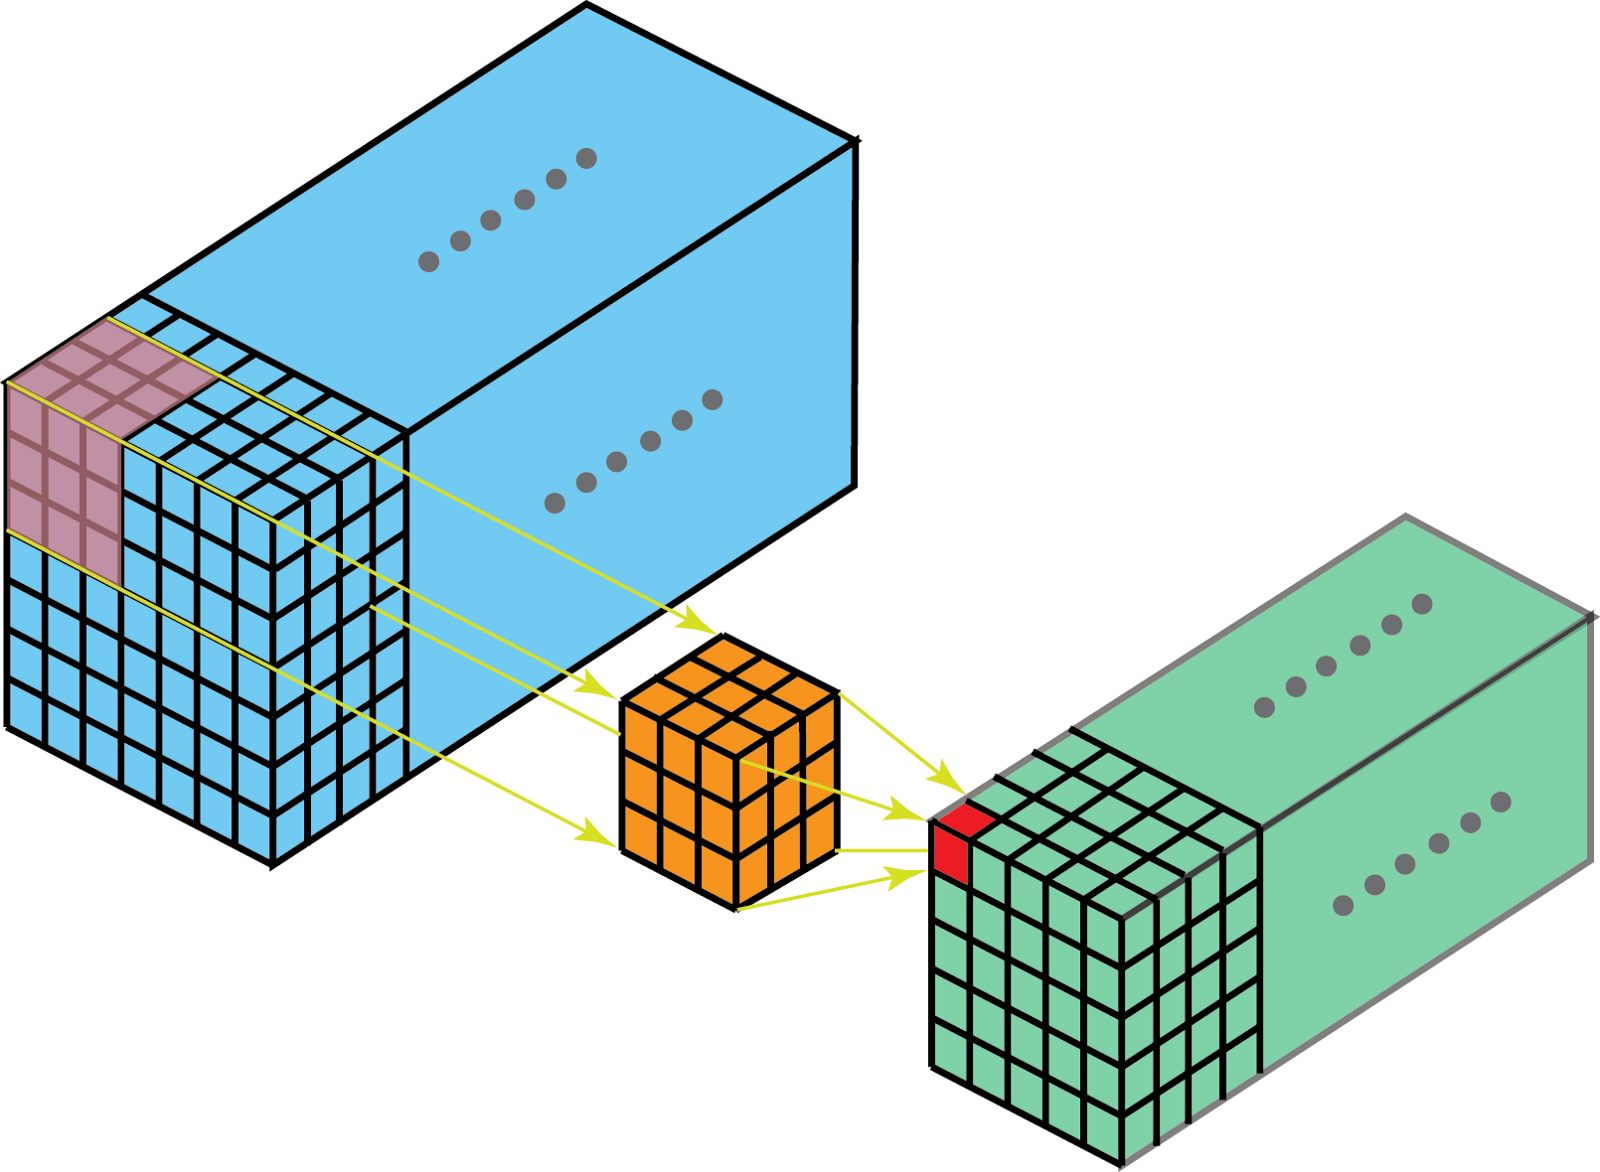
\includegraphics[width=2.5in]{figures/chapter5/3d_conv.png}
    \caption{A schematic depiction of a 3D convolution for use in a CNN.}
    \label{fig:3d_conv}
\end{figure}

Including other types of information like timing and cell quality could further improve network performance. There are important questions that must be addressed before an image-based electron ID could be fully incorporated into the ATLAS software flow. This includes how to handle the barrel to endcap transition when constructing images and understanding whether including $\eta$ values allows the network to account for the fact that the layer images do not actually lie directly on top of each other in the physical detector. Furthermore, as discussed in Section \ref{sec:data_vs_mc} the ultimate goal is to develop an algorithm that is fully data-driven. This presents additional challenges when training ML algorithms as they typically require very high training sample purity in order to achieve reasonable performance. Methods for purifying the data-sets currently used for the LH-based ID without biasing any kinematics are being explored.
